
\setcounter{chapter}{4}
\chapter{The Laplace Transform and Applications}\label{ch:Laplace Transform}
	

\mtcsetoffset{minitoc}{-1em}
% \mtcsetpagenumbers{minitoc}{off}

\minitoc %This TOC should only show the two subsubsection below!

\section{The Laplace Transform}\label{chap7:section1}



Consider a forced oscillator, as discussed in Section~\ref{subsection:spring-mass} of Chapter~\ref{chap:higher-order}, described by the equation  
\begin{equation}\label{chap7:01}
	y''(t) + \omega^2 y(t) = f(t); \quad  y(0) = 0,\; y'(0)= 0,
\end{equation}  
where \( f(t) \) is an impulsive  force. At \(t =0,\) the mass is at rest at its equilibrium position. At time \( t = a \), the mass experiences a sharp, brief downward impact, such as a hammer strike, modeled by an the impulsive force \( f(t) .\) 
An impulsive force of this nature is commonly modeled by using an idealized mathematical object, called the   \textbf{\textit{Dirac delta}} ``function'' denoted by $\delta (t-a),$ which is characterized by the following  properties:

\begin{enumerate}[label= (\roman*)]
	\item \( \delta(t - a) = 0 \) for all \( t \ne a \); and
%	\item \( \int_{-\infty}^\infty \delta(t - a)\, dt = 1 \); and
	\item \( \int_{-\infty}^\infty \delta(t - a)\, g(t)\, dt = g(a) \) for any function \( g \) continuous on an open interval containing \( a \).
\end{enumerate}
We note  that when $g(t) =1$ in (ii), we obtain 
\( \int_{-\infty}^\infty \delta(t - a)\, dt = 1 \).
Based on the  properties (i) and (ii) characterizing \( \delta(t - a) \), it is important to recognize that \( \delta(t - a) \) is not a  function in the usual sense; rather it is a typical example of \textit{generalized functions} or \textit{distributions} which were first developed rigorously  by Sergei Sobolev in 1936 and later in 1950s by Laurent Schwartz who is known to have given the most definitive and systematic development of the theory of distributions. For an elegant introduction to  distribution theory with application, the reader is referred to  Zemanian\footnote[1]{A.~H. Zemanian, {\it Distribution theory and transform analysis}, second edition, Dover, New York, 1987; MR0918977}.

 The Dirac delta function is particularly useful for modeling  phenomena involving instantaneous or localized effects, such as a lightning strike, a point heat explosion, or the sudden burst of dye at a specific location. Because of the properties (i) and (ii), the Dirac delta function \( \delta(t - a) \) is said to be concentrated at $t=a.$ 


Mathematically,  \( \delta(t - a) \) can be interpreted as the limit  of a sequence of approximating impulse functions.  One such approximation is given by  
 \[
 d_{a, \varepsilon}(t) = \begin{cases}
	 \dfrac{1}{\varepsilon} &\text{if } a \le t \le a + \varepsilon \\
	0 &\text{otherwise},
	 \end{cases}
 \]
 which represents a  pulse of height \( 1/\varepsilon \) and width \( \varepsilon>0 \), centered at \( t = a \). 
 
% \textcolor{red}{Open this figure later}
 \begin{figure}[h]
 	\centering
 	\begin{tikzpicture}[scale=1.5]
 		% Axes
 		\draw[->] (-0.5,0) -- (4,0) node[right] {$t$};
 		\draw[->] (0,-0.2) -- (0,2) node[above] {$d_{a,\varepsilon}(t)$};
 		
 		% Parameters
 		\def\a{1}
 		\def\eps{0.5}
 		\def\height{1.5} % 1 / eps
 		
 		% Rectangle function
 		\draw[thick, blue] (0,0) -- (\a,0)
 		-- (\a,\height) -- ({\a+\eps},\height)
 		-- ({\a+\eps},0) -- (4,0);
 		
 		% Labels
 		\draw[dashed] (\a,0) -- (\a,\height);
 		\draw[dashed] ({\a+\eps},0) -- ({\a+\eps},\height);
 		
 		\node[below] at (\a,0) {$a$};
 		\node[below] at ({\a+\eps},0) {$a+\varepsilon$};
 		\node[left] at (0,\height) {$\frac{1}{\varepsilon}$};
 		
 	\end{tikzpicture}
 \end{figure}
 

 
 As \(\varepsilon \to 0 \), this pulse becomes increasingly narrow and tall, concentrating its effect at \( t = a \), i.e.,  
 \begin{equation}\label{chap7:02}
 	\lim\limits_{\varepsilon\to 0} d_{a, \varepsilon}(t) = \begin{cases}
 	\infty &\mbox{if } t=a\\
 	0&\text{otherwise},
 \end{cases}\end{equation}
 while maintaining a total area of 1—mirroring the property (ii) of \( \delta(t - a) \), i.e.,
 \[\int_{-\infty}^\infty d_{a, \varepsilon}(t) \, dt = \frac{1}{\varepsilon} \varepsilon=1,\]
 so that 
 \begin{equation}\label{chap7:03}
 	\lim\limits_{\varepsilon\to 0} \int_{-\infty}^\infty d_{a, \varepsilon}(t) \, dt =1.
 	\end{equation}
 Furthermore, if $g$ is continuous from right at $t=a$,  then
  \begin{equation}\label{chap7:04}
 	\lim\limits_{\varepsilon\to 0} \int_{-\infty}^\infty d_{a, \varepsilon}(t) \, g(t) = 	\lim\limits_{\varepsilon\to 0}\frac{1}{\varepsilon} \int_a^{a+\varepsilon}  g(t) \, dt = \lim\limits_{\varepsilon\to 0} g(a+\varepsilon) = g(a)
 \end{equation}
by using the l'H\"opital's rule and the continuity of $g$ at $t=a$ from right. 

 By formally interchanging the limit and the integral in both (\ref{chap7:03}) and (\ref{chap7:04}), an operation which needs justification  in integration theories, we obtain  
\begin{equation}\label{chap7:05}
	\int_{-\infty}^\infty\lim\limits_{\varepsilon\to 0} d_{a, \varepsilon}(t)\, dt = 1
\end{equation}  
and 
\begin{equation}\label{chap7:06}
	 \int_{-\infty}^\infty \lim\limits_{\varepsilon\to 0} d_{a, \varepsilon}(t) \, g(t)\, dt  = g(a).
	\end{equation}
 Thus, we observe in (\ref{chap7:02}) and (\ref{chap7:06})  that  
 \( \lim\limits_{\varepsilon \to 0} d_{a, \varepsilon}(t) \) exhibits the same  properties (i) and (ii) that characterize \( \delta(t - a) \), and therefore \( \delta(t - a) \) can be interpreted as the limit of a sequence of functions that approximate an impulsive behavior.   
We recognize that 
\(
\lim\limits_{\varepsilon \to 0} d_{a, \varepsilon}(t)
\)
also does not define a function on $(-\infty, \infty)$ in the classical sense because its value at $t=a$ is $\infty.$ Instead, the limit is understood as a generalized function, or a distribution, because of the way it operates primarily through its action on other functions within integrals, as described by the property (ii) and motivated by (\ref{chap7:06}).
 


   By using the property (ii), we  find that for all $s$ in $(-\infty,  \infty),$ we have 
\begin{equation}\label{chap7:07}
	\int_{-\infty}^\infty \delta(t - a)\, e^{-st}\, dt = e^{-as} \end{equation}
for all real numbers $s.$
From this point onward, we will focus on the case where \( a \ge 0 \) and \( t \ge 0 \). Under this assumption,  (\ref{chap7:07}) reduces to  
 \begin{equation}\label{chap7:08}
	 \int_0^\infty \delta(t - a)\, e^{-st}\, dt = e^{-as}
	 \end{equation}
 for all real values of \( s \).  
 This integral is known as the \textbf{\textit{Laplace transform}} (see Definition~\ref{chap7:Laplace})of the Dirac delta function \( \delta(t - a) \),  denoted by  
 \[
 \mathscr{L}\{\delta(t - a)\} = e^{-as}.
 \]  
 In particular, when $a=0$ we have 
 \[
 \mathscr{L}\{\delta(t)\} = 1.
 \]
 
 

 The main objective of this chapter is to develop a method for solving initial value problems such as (\ref{chap7:01} in which $f(t)$ is either discontinuous or involves the Dirac delta functions.The methods of undetermined coefficients and  variation of parameters are not relevant to (\ref{chap7:01}) with $f(t) = \delta (t-a)$  because the calculus of distributions is beyond the scope of this book.   In particular,  we do not have a meaning of $y''$ in this case.
 
 Being motivated from  (\ref{chap7:08}) with the Dirac delta function \(\delta(t - a)\) in the integrand, we first define the Laplace transforms of classical functions defined on $[0, \infty).$

\begin{definition}[Laplace Transform]\label{chap7:Laplace}
Let $f:[0, \infty)\to\mathbb R$ be a function. The Laplace transform  of $f$  is a function $F(s)$, denoted commonly by $\mathscr{L}\{f(t)\}$, defined by
 \[F(s):=\int_0^\infty f(t)\, e^{-st} \, dt\]  for those $s$ for which the integral converges.
\end{definition}






The symbol $\mathscr{L}$ represents a transformation that maps an input function $f$ of the variable $t$ (usually time) to an output function $F$ of the variable $s$ (usually involving frequency when 
$s$ is a complex number). This action of the transformation is depicted in the figure below.


	
%	\begin{tikzpicture}[node distance=3cm, auto]
%		% Nodes
%		\node (input) [draw, rectangle, minimum height=1cm, minimum width=2.5cm] {\(f(t)\)};
%		\node (L) [draw, circle, right of=input, node distance=3.5cm] {\(\mathscr{L}\)};
%		\node (output) [draw, rectangle, right of=L, node distance=3.5cm, minimum height=1cm, minimum width=2.5cm] {\(F(s)\)};
%		
%		% Arrows
%		\draw[->, thick] (input) -- (L);
%		\draw[->, thick] (L) -- (output);
%		
%		% Labels
%		\node[below of=input, node distance=.75cm] {$t$ domain};
%		\node[below of=output, node distance=.75cm] {$s$ domain};
%	\end{tikzpicture}
	
	% \textcolor{red}{Open this figure later}
	\begin{center}
	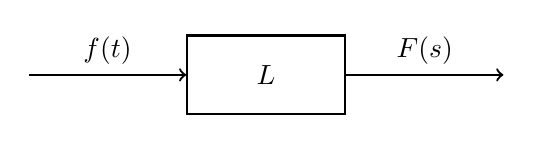
\begin{tikzpicture}[node distance=2.5cm, thick]
		% Draw the box
		\node[draw, minimum width=2cm, minimum height=1cm, align=center] (laplace) {$\mathscr{L}$};
		
		% Input arrow and label
		\draw[->] ([xshift=-2cm]laplace.west) -- (laplace.west) node[midway, above] {$f(t)$};
		
		% Output arrow and label
		\draw[->] (laplace.east) -- ([xshift=2cm]laplace.east) node[midway, above] {$F(s)$};
	\end{tikzpicture}
\end{center}


The variable \( s \) in the definition of the Laplace transform can, in general, be a complex variable; however, in the current chapter,  we will restrict  \( s \) to a real variable.


 Before we begin using Laplace transforms to solve initial value problems, we  compute the Laplace transforms of several common functions that appeared in the previous chapters.

\begin{example}
Compute $\mathscr{L}\{e^{at}\}$ for $a\ne 0.$
\end{example}
\begin{solution}
	By Definition~\ref{chap7:Laplace}, we have
\begin{equation*}
	\begin{split}
		\mathscr{L} \bigl\{e^{at}\bigr\}
		=\int_0^\infty e^{at} \,e^{-st}  \, dt
		&= \lim_{h\to\infty}\int_0^h e^{(a-s)t} \, dt\\
	 	&=\lim_{h\to\infty}\left[ \frac{e^{(a-s)t}}{a-s} \right]_0^h\\
	 	&=\lim_{h\to\infty}\frac{e^{(a-s)h}}{a-s}- \frac{1}{a-s}\\
		& = \frac{1}{s-a}
		\end{split}
\end{equation*} for all $s>a.$ The improper integral converges only for $s>a.$ Thus, 
\[\boxed{\mathscr{L} \bigl\{e^{at}\bigr\}= \frac{1}{s-a}\quad \text{ for all } s>a.}\qedhere\]
\end{solution}


\begin{example}
	Compute $\mathscr{L}\{1\}.$ 
\end{example}
\begin{solution}
	By Definition~\ref{chap7:Laplace}, we have
	\begin{equation*}
		\mathscr{L} \{1\} = \int_0^\infty e^{-st} \, dt
		=
		\lim_{h\to\infty}
		\left[ \frac{e^{-st}}{-s} \right]_0^h
		=
		\lim_{h\to\infty}
		\left( \frac{e^{-sh}}{-s} - \frac{1}{-s} \right)
		= \frac{1}{s} 
	\end{equation*}
	for $s>0.$ The improper integral converges only for $s>0.$ 
	Thus, 
	\[\boxed{\mathscr{L} \{1\} = \frac{1}{s}\quad \text{ for all } s>0.}\qedhere\]
\end{solution}
In the sequel, the expression \(
\left[ g(t)\right]_0^\infty\) will be tacitly used for
\(\lim\limits_{h\to\infty}
\left[ g(t)\right]_{0}^h.\)
 
 
 
 \begin{example}
 Compute $\mathscr{L}\{t\} .$
 \end{example}
 \begin{solution}
 
 	By Definition~\ref{chap7:Laplace}, we have
\begin{equation*}
	\begin{split}
		\mathscr{L} \{t\}
		& = \int_0^\infty t\,e^{-st}  \, dt \\
		& =
		\left[ \frac{-te^{-st}}{s} \right]_0^\infty
		+
		\frac{1}{s}
		\int_0^\infty e^{-st} \,dt \qquad \text{(integration  by parts)} \\
		& =
		0
		+
		\frac{1}{s}
		\left[ \frac{e^{-st}}{-s} \right]_0^\infty \\
		& =
		\frac{1}{s^2}
	\end{split}
\end{equation*}
 for $s>0.$ The improper integral converges only for $s>0.$ Thus, 
 \[\boxed{\mathscr{L} \{t\} = \frac{1}{s^2}\quad \text{ for all } s>0.}\qedhere\]
\end{solution}


\begin{example}
	Compute $\mathscr{L}\{t^2\} .$
\end{example}
\begin{solution}
	By Definition~\ref{chap7:Laplace}, we have
		\[
	\mathscr{L}\{t^2\} = \int_0^\infty e^{-st} t^2 \, dt.
	\] 
To use integration by parts, put \(
	u = t^2\)  and \(dv = e^{-st} dt\). Then \( du = 2t\,dt\) and 
	\(v = -\frac{1}{s}e^{-st}\). Then
\begin{equation*}
	\begin{split}
	\mathscr{L}\{t^2\} = \int_0^\infty t^2 e^{-st} dt
						&= \left[ -\frac{1}{s} t^2 e^{-st} \right]_0^\infty - \int_0^\infty \left(-\frac{1}{s}e^{-st}\right) 2t dt\\
						&=-\frac{1}{s^2}\lim_{t\to\infty}t^2 e^{-st} + 0+ \frac{2}{s}\int_0^\infty t e^{-st}\, dt\\
						&=\frac{2}{s} \mathscr{L}\{t\}\\
						&= \frac{2}{s^3}
	\end{split}
\end{equation*}
for $s>0$. Here, we used the limit
\[\lim_{t\to\infty}t^2 e^{-st} =0\] which can be evaluated by using the l'H\"opital's rule. Also, the improper integral defining \(\mathscr{L}\{t^2\}\) converges only for $s>0.$ Thus, 
\[\boxed{\mathscr{L} \{t\} = \frac{2}{s^3}\quad \text{ for all } s>0.}\qedhere\]
\end{solution}


\begin{example}
	Compute $\mathscr{L}\{t^3\} .$
\end{example}
\begin{solution}
By repeatedly using integration by parts and the l'H\"opital's rule, we obtain
\[\boxed{\mathscr{L} \{t^3\} = \frac{3!}{s^4}\quad \text{ for all } s>0.}\qedhere\]
\end{solution}

The computation of \(\mathscr{L}\{t^n\}\) for any positive integer $n$ follows the same procedure as shown in the next example.

\begin{example}
	Compute $\mathscr{L}\{t^n\} $ for any positive integer $n.$
\end{example}
\begin{solution}
	By integration by parts and the l'H\"opital's rule, we obtain
	\[\mathscr{L} \{t^n\} = \frac{n}{s}{\mathscr{L} \{t^{n-1}\}}\quad \text{ for all } s>0.\]
	Using this recursive relation, we obtain
	\[\begin{split}
		\mathscr{L} \{t^n\} &= \frac{n}{s}\left(\frac{n-1}{s}\right){\mathscr{L} \{t^{n-2}\}}\\
		&= \frac{n}{s}\left(\frac{n-1}{s}\right)\left(\frac{n-2}{s}\right){\mathscr{L} \{t^{n-3}\}}\\
		&\quad \vdots\\
			&= \frac{n}{s}\left(\frac{n-1}{s}\right)\left(\frac{n-2}{s}\right)\cdots \frac{3}{s}\; \frac{2}{s}{\mathscr{L} \{t\}}\\
			&=\frac{n}{s}\left(\frac{n-1}{s}\right)\left(\frac{n-2}{s}\right)\cdots \frac{3}{s}\; \frac{2}{s}\;\frac{1}{s^2}\\
			&=\frac{n!}{s^{n+1}}
	\end{split}
	\]
	for $s>0$.  As in the previous cases, the improper integral defining \(\mathscr{L}\{t^n\}\) converges only for $s>0.$ Thus, 
	\[\boxed{\mathscr{L} \{t^n\} = \frac{n!}{s^{n+1}}\quad \text{ for all } s>0.}\qedhere\]
\end{solution}

\begin{example}
	Compute $\mathscr{L}\{\sin(kt)\}$ for any fixed constant $k.$
\end{example}
\begin{solution}

	By the definition of  the Laplace transform of \( \sin(kt) \), where \( k \) is a constant, we have
	
	\[
	\mathscr{L}\{\sin(kt)\} = \int_0^\infty e^{-st} \sin(kt) \, dt.
	\]
By using integration by parts,  we have 
\[
\int e^{-st} \sin(kt) \, dt = -\frac{e^{-st}}{s^2 + k^2}\left(s \sin(kt) + k \cos(kt)\right)   + C,
\]
where $C$ is an arbitrary constant.
Then 

\[
\int_0^\infty e^{-st} \sin(kt) \, dt =-\left[\frac{e^{-st}}{s^2 + k^2}\left(s \sin(kt) + k \cos(kt)\right) \right]_0^\infty.
\]
Since $e^{-st} \to 0$  as $t\to\infty$ and $s \sin(kt) + k \cos(kt)$ is bounded, we have
\[
\lim_{t \to \infty} e^{-st}\left( s \sin(kt) + k \cos(kt) \right)  = 0\] for $s>0.$ The improper integral converges only for $s>0$ when $k\ne 0.$
Therefore, we have
\[
\boxed{\mathscr{L}\{\sin(kt)\} = \frac{k}{s^2 + k^2} \quad \text{ for all } s>0.}\qedhere
\]
\end{solution}


\begin{example}
	Compute $\mathscr{L}\{\cos(kt)\}$ for any fixed constant $k.$
\end{example}
\begin{solution}
	By using integration by parts,  we have 
	\[
\int e^{-st} \cos(kt) \, dt = \frac{e^{-st}}{s^2 + k^2} \left( -s \cos(kt) + k \sin(kt) \right) + C,
	\]
	where $C$ is an arbitrary constant.
	Then 
	
	\[
	\int_0^\infty e^{-st} \cos(kt) \, dt =\left[\frac{e^{-st}}{s^2 + k^2}\left(-s \cos(kt) + k \sin(kt)\right) \right]_0^\infty.
	\]
	Since $e^{-st} \to 0$  as $t\to\infty$ and $-s \cos(kt) + k \sin(kt)$ is bounded, we have
	\[
	\lim_{t \to \infty} e^{-st}\left( -s \cos(kt) + k \sin(kt) \right)  = 0\] for $s>0.$ The improper integral converges only for $s>0.$ 
	Therefore, 
	we obtain
	\[
	\boxed{\mathscr{L}\{\cos(kt)\} = \frac{s}{s^2 + k^2}} \quad \text{ for all } s>0.\qedhere
	\]
\end{solution}
A simple but useful example of a discontinuous function is
the \textbf{\textit{unit step function}} $\mathcal{U}$, also  known as the \textbf{\textit{Heaviside}} function (named in honor of the English mathematician, engineer, and physicist Oliver Heaviside (1850--1925)). It is defined on $(-\infty, \infty)$ by
\[
\mathcal{U}(t) =
\begin{cases}
	0 & \text{if } t < 0, \\
	1 & \text{if } t \ge 0.
\end{cases}
\]

%\textcolor{red}{Open this figure later}
\begin{figure}[h]
	\centering
	\begin{tikzpicture}[scale=.75]
		\tkzInit[xmin=-1,xmax=4,ymin=-0.5,ymax=1.5]
		\tkzSetUpAxis[line width=1pt,tickwd=0pt,ticka=0pt,tickb=0pt]
		\tkzDrawXY
		
		% Draw U(t) = 0 for t < 0
		\draw[thick, blue] (-1,0) -- (0,0);
		\filldraw[blue,thick] (0,0) circle (2pt); 
		\filldraw[white] (0,0) circle (1.5pt); % open circle at t = 0
		
		% Draw U(t) = 1 for t >= 0
		\draw[thick, blue] (0,1) -- (4.5,1);
		\filldraw[blue] (0,1) circle (2pt); % filled circle at t = 0
		
		% Label the step
		\node[above right] at (0.1,1) {\(\mathcal{U}(t)\)};
	\end{tikzpicture}
	\caption{The unit step function \(\mathcal{U}(t)\)}
\end{figure}
The unit step function with the jump discontinuity at $t= a$ is given by 
\[
\mathcal{U}(t-a) =
\begin{cases}
	0 & \text{if } t < a, \\
	1 & \text{if } t \ge a,
\end{cases}
\]
and its graph is shown below.
%\textcolor{red}{Open this figure later}
\begin{figure}[h]
	\centering
	\begin{tikzpicture}[scale=.9]
		\tkzInit[xmin=-1,xmax=4,ymin=-0.5,ymax=1.5]
		  \tkzSetUpAxis[line width=1pt,tickwd=0pt,ticka=0pt,tickb=0pt]
		\tkzDrawXY
		
		% Draw U(t) = 0 for t < 0
		\draw[thick, blue] (-1,0) -- (2,0);
		\filldraw[blue,thick] (2,0) circle (2pt); 
		\filldraw[white] (2,0) circle (1.5pt); % open circle at t = 0
		
		% Draw U(t) = 1 for t >= 0
		\draw[thick, blue] (2,1) -- (4.5,1);
		\filldraw[blue] (2,1) circle (2pt); % filled circle at t = 0
		
		% Label the step
		\node[above right] at (2.1,1) {\(\mathcal{U}(t-a)\)};
		\node[above right] at (1.7,-0.6) {\(a\)};
	\end{tikzpicture}
	\caption{The unit step function \(\mathcal{U}(t-a)\)}
\end{figure}


\begin{example}\label{chap7:example-heaviside}
	Compute $\mathscr{L}\{\mathcal{U}(t-a)\}$ for  $a\ge 0.$
\end{example}

\begin{solution}
	By Definition~\ref{chap7:Laplace}, we have
	\begin{equation*}
		\mathscr{L} \bigl\{ \mathcal{U}(t-a) \bigr\}
		=
		\int_0^{\infty} e^{-st} \mathcal{U}(t-a) \, dt
		=
		\int_a^{\infty} e^{-st} \, dt
		=
		\left[ \frac{e^{-st}}{-s} \right]_a^\infty \\
		=
		\frac{e^{-as}}{s} 
	\end{equation*}
	 for $s>0.$   Also, the improper integral defining \(\mathscr{L}\{\mathcal{U}(t-a)\}\) converges only for $s>0.$ Thus, 
	 \[\boxed{\mathscr{L} \{\mathcal{U}(t-a)\} = \frac{e^{-as}}{s} \quad \text{ for all } s>0.}\qedhere\]
\end{solution}


To model situations in applications where an external force or source begins acting only after time \( t = a \), we analyze the effect of shifting the source function along the \( t \)-axis.



Suppose the function \( f(t) \) is intended to take effect only after time \( t = a \). In that case, we define a new function \( g(t) \) as  
\[
g(t) =\begin{cases}
	f(t-a) & \text{if } t \ge a,\\
	0 & \text{if } t < a,
\end{cases}
\]
whose graph is shown below in comparison to the graph of $f(t).$

%\textcolor{red}{Open this figure}
\begin{center}
	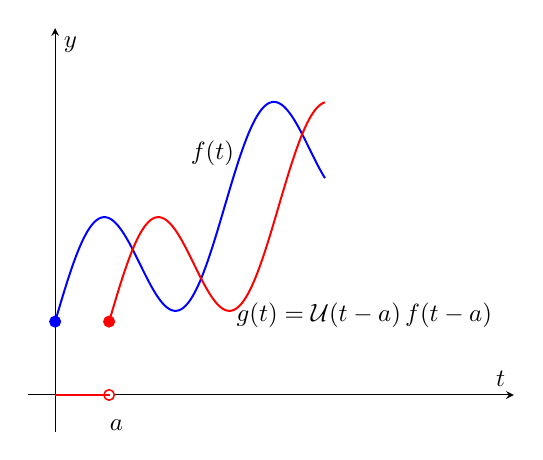
\begin{tikzpicture}[scale=.9]
		\begin{axis}[
			axis lines = middle,
			xlabel = $t$, ylabel = $y$,
			xmin = -1, xmax = 17,
			ymin = -0.5, ymax = 5,
			samples = 200,
			xtick = \empty,
			ytick = \empty,
			legend style={at={(0.5,-0.15)}, anchor=north},
			grid = both
			]
			% Original function f(t)
			\addplot[blue, thick, domain=0:10] {1+sin(deg(x))+0.25*x};
			%\addlegendentry{$y= f(t)$}
		% Draw U(t) = 0 for t < 0
			
	
			\filldraw[red,thick] (2,0) circle (2pt); 
			\filldraw[white] (2,0) circle (1.5pt);
			
			%\draw[thick, red] (-3,0) -- (0,0);
			\filldraw[blue,thick] (0,1) circle (2pt); 
			\filldraw[red,thick] (2,1) circle (2pt); 
			%\filldraw[white] (2,1) circle (1.5pt);
			
			% Shifted function g(t) = f(t-a) for t >= a, else 0
			\addplot[red, thick, domain=0:2] {0};
			\addplot[red, thick, domain=2:10] {1+sin(deg(x - 2))+0.25*(x-2)};
			\node[above right] at (4.7,3) {\(f(t)\)};
			\node[above right] at (6.4,.8) {\(g(t) =\mathcal{U}(t-a)\,f(t-a)\)};
			\node[above right] at (1.7,-0.6) {\(a\)};

			%\addlegendentry{$g(t) = f(t - a)$ for $t \ge a$}
		\end{axis}
	\end{tikzpicture}
\end{center}
It is clear that $g(t) = \mathcal{U}(t-a) f(t-a)$ for $t\ge 0.$



\begin{example}[Shifting on the $t-$axis]\label{shiting-on-t-axis}
	 Suppose \( F(s) \) is the Laplace transform of \( f(t) \). Compute  \(\mathscr{L} \{\mathcal{U}(t - a)\, f(t - a) \}\) where \( a \ge 0 \).
\end{example}
\begin{solution}
By the definition of the Laplace transform, we have
	\[
	\mathscr{L}\{\mathcal{U}(t - a)\, f(t - a)\} = \int_0^\infty e^{-st} \mathcal{U}(t - a)\, f(t - a)\, dt.
	\]
	Since \( \mathcal{U}(t - a) = 0 \) for \( t < a \), the lower limit of the integral can be shifted to \( a \), i.e., 
	\[
	\mathscr{L}\{\mathcal{U}(t - a)\, f(t - a)\} = \int_a^\infty e^{-st} f(t - a)\, dt.
	\]
  Put \(t - a =u\). Then  \(t = a+u\) and \(dt = du.\)
	When \( t = a  \), \( u = 0 \), and as $t\to \infty$, $u\to\infty$, so the integral becomes
	\[\int_0^\infty e^{-s(a+u)} f(u)\, du = e^{-as} \int_0^\infty e^{-su} f(u)\, du
	\]
	
	\[
	= e^{-as} F(s).
	\]
	Thus,
	\[
	\boxed{\mathscr{L}\{\mathcal{U}(t - a)\, f(t - a)\} = e^{-as} F(s).}
	\]
	The shifted function $f(t-a)$ is technically written $f(t)\vert_{t\to t-a}.$  Thus, we can write
	\[
	\boxed{
		\mathscr{L}\{\mathcal{U}(t)\, f(t)\vert_{t\to t-a}\} = e^{-as} F(s).
	}\qedhere
	\]
\end{solution}

 The linearity  of the Riemann integration yields the linearity of the Laplace transform operator 
\(\mathscr{L}\), as stated in the following theorem.

\begin{theorem}[Linearity of \(\mathscr{L}\)]
	Let $f$ and $g$ be functions defined on $[0, \infty)$ whose   Laplace transforms exist for all $s>s_0$, where $s_0$ is some real number. Then, for any constants $a$ and $b$, the function $h$ defined by $h(t) = af(t) + bg(t)$ also has Laplace transform $H(s)$ for all $s> s_0,$ and  we have
	\[\mathscr{L}\left\{ {af\left( t \right) + bg\left( t \right)} \right\} = a\,\mathscr{L}\left\{f (t)\right\} + b\,\mathscr{L}\left\{g (t)\right\},\] i.e.,
	\[H(s) = aF(s) + bG(s), \quad s>s_0.\]
\end{theorem} 

 \subsection{When does the Laplace transform exist?}
 An immediate question one might ask is: what sort of functions $f(t)$ actually have Laplace transforms according to Definition~\ref{chap7:Laplace}?
To answer this in the context of the Riemann integration, we note that $F(s) =\mathscr{L}\{f(t)\}$ is the limit of the definite integrals 
 	\[\int_0^b  e^{-st} f(t)\, dt\] 
 	as $b\to\infty$ whenever it exists,  and therefore
  $f(t)$ cannot have a vertical asymptote at any point $t =b$. To avoid any chances for vertical asymptotes, we  take $f(t)$ to be \textbf{\textit{piecewise continuous}} on $[0, \infty).$ A piecewise continuous function on \([0,\infty)\)  is one which can have at most a finite number of jump discontinuities on each closed subinterval \([a, b]\) of \([0,\infty)\).  An example of a piecewise continuous function is depicted in the figure below. \\
  
 %\textcolor{red}{Open this figure later}
  	\begin{figure}[h]
  \centering
  	\begin{tikzpicture}[scale=0.7]
  		\tkzInit[xmin=0,xmax=10,ymin=-1.5,ymax=4]
  		\tkzDrawXY
  		
  		% First piece: f(t) = t on [0,2)
  		\draw[domain=0:2, thick, blue] plot (\x,\x);
  		
  		% Open circle at (2,2) to indicate discontinuity
  		\filldraw[blue, thick] (0,0) circle (2pt);
  		\filldraw[white] (2,2) circle (2pt);
  		\draw[blue, thick] (2,2) circle (2pt);
  		
  		% Second piece: f(t) = 3 on [2,4)
  		\draw[thick, blue] (2,3) -- (4,3);
  		\filldraw[white] (4,3) circle (2pt);
  		\draw[blue, thick] (4,3) circle (2pt);
  		\filldraw[blue,thick] (2,3) circle (2pt);
  		
  		% Third piece: f(t) = sin(t) on [4,6]
  		\draw[domain=4:6, samples=100, thick, blue] plot (\x,{sin(deg(\x))});
  		\filldraw[blue,thick] (4,{sin(deg(4))}) circle (2pt);
  		\filldraw[white] (6,{sin(deg(6))}) circle (2pt);
  		\draw[blue, thick] (6,{sin(deg(6))}) circle (2pt);
  		
  	
  		% Fourth piece: f(t) = 0 on (6,10]
  		\filldraw[thick, blue] (6,0) -- (8,0);
  		\filldraw[blue,thick] (6,0) circle (2pt);
  		
  		\filldraw[white] (8,0) circle (2pt);
  		\draw[blue, thick] (8,0) circle (2pt);
  		
  		\draw[domain=8:10, samples=100, thick, blue,->] plot (\x,{\x-6});
  		\filldraw[blue, thick] (8,2) circle (2pt);
  	\end{tikzpicture}
  		\caption{An example a piecewise continuous function}
  	\end{figure}
  	
  \noindent However,  the condition that $f$ be piecewise continuous on $[0, \infty)$ would not be sufficient for the existence of its  Laplace transform. For instance,  the function $f(t)= e^{t^2}$ does not have its Laplace transform. In fact, for each fixed number $c$, there exists $t_0$ such that $t^2> ct$ for  all  $t\ge t_0,$ and this implies that  
  \[ \int_{t_0}^b  e^{-st} e^{t^2}  \, dt = \int_{t_0}^b  e^{t^2-st}  \, dt >  \int_{t_0}^b  e^{(c-s)t}  \, dt.\] This results in
   \[\int_0^\infty  e^{-st} e^{t^2}  \, dt\ge \int_{t_0}^\infty  e^{-st} e^{t^2}  \, dt \ge  \int_{t_0}^\infty  e^{(c-s)t}  \, dt = \infty\] for all $s\le c.$ This holds for every number $c$, and therefore $f(t) = e^{t^2}$ does have its Laplace transform. From this example, we observe that $e^{-st}$ must control the growth property of $f(t)$ as $t\to\infty$ for the existence its Laplace transform. In particular, in addition to the piecewise continuity, 
 if $f(t)$ is of an \textbf{\textit{exponential order}} as $t\to\infty,$ i.e., if  there exist constants $\alpha$, $M>0,$  and $t_0>0$ such that 
  \[ \abs{f(t)} \le M e^{\alpha t} \quad \mbox{ for all } t\ge t_0,\]
  then, for all $b\ge t_0$, we find
   
  \[\abs{\int_0^b  e^{-st} f(t) \, dt} \le \int_0^b  e^{-st} \abs{f(t)} \, dt\le \int_0^b  e^{-st} Me^{\alpha t} \, dt =M\int_0^b e^{-(s-\alpha)t}\, dt.\]
Consequently, 
  \[F(s) =\int_0^\infty  e^{-st} f(t) \, dt\] exists for $s>\alpha.$ 
We formalize all these ideas together in the following existence theorem.
 
 \begin{theorem}[Existence of the Laplace Transform]
 	Let $f$ be a piecewise continuous function on $[0,\infty)$ and of an exponential order as $t\to\infty$.  Then $F(s)=\mathscr{L}\{f(t)\}$ exists.
 \end{theorem}
% We remark that there exist continuous functions that are not of exponential order at infinity and  have no Laplace transform. For example, the function  $f(t)= e^{t^2}$ on $[0, \infty)$ does not have Laplace transform. In fact, for any real number $s$, we have
% \[e^{t^2} e^{-st}  = e^{t(t-s)}\ge 1\] whenever $t\ge s.$ This implies 
% \[\int_0^be^{t^2} e^{-st}\, dt = \int_0^b e^{t(t-s)}\, dt \ge  b.\] 
% Letting $b\to \infty,$ we see that \[\int_0^\infty e^{t^2} e^{-st}\, dt\] diverges, that is, $f$ does not have its Laplace transform.
% 
% \begin{remark}$\empty$
% 	\begin{enumerate}[label={(\roman*)}, noitemsep]
% 		\item  The conditions that $f$ be piecewise continuous on $[0, \infty)$ and of exponential order as $t \to \infty$ are sufficient, but not necessary, for the existence of the Laplace transform. For instance, consider the function 
% 		\[f(t) = \begin{cases}
% 			t^{-1/2} & \text{if } t>0,\\
% 			0&\text{if } t=0.
% 		\end{cases}\]
% 	Since $f$ is not continuous on any interval that contains $0,$ it follows that $f$ is not piecewise continuous on $[0, \infty),$  but $f$ is of exponential order as $t\to \infty.$
% 	
% 	
% 	
% 		
% 		
% 		\item There exist continuous functions that are not of exponential order at infinity and  have no Laplace transform.
% 	\end{enumerate}
% \end{remark}

 
 
We are interested in whether two different functions can have the same Laplace transform.  Trivial examples of functions that have the same Laplace transform are $g(t) =\mathcal U(t-a)$ with  $a>0$ and $h(t)$ defined by
 \[
 h(t) =\begin{cases}
 	1& \text{if } t > a,\\
 	0 & \text{if } t \le a.
 \end{cases}
 \]
 Note that $g(a) = 1$ and $h(a)= 0,$ and  $g(t) = h(t)$ for all $t\ne a.$ Since $g$ and $h$ differ only at one single point in $[0, \infty),$  it follows, by the definition of the Laplace transform, that \[\ds G(s) = H(s) = \frac{e^{-s}}{s}\] for $s>0.$ This implies that \(\mathscr{L}\) is not a one-to-one function from functions \(f(t)\) of the variable \(t\) to functions \(F(s)\) of the variable \(s\).
 
 \subsection{Inverse Laplace Transforms}\label{chap7:subsection1}

 As mentioned at the end of Section~\ref{chap7:section1}, the forced oscillator (\ref{chap7:01}) cannot be solved using the methods from previous chapters when \( f \) is a Dirac delta. Even if \( f \) is only piecewise continuous, the earlier methods can become quite tedious to apply. The Laplace transform method provides a more efficient approach, and this method involves taking the Laplace transform of a linear differential equation and converting it into an algebraic equation. After solving the algebraic equation in the $s$-domain for the Laplace transform of the solution function, we then apply the one-to-one property of the Laplace transform to return to the solution in the $t-$domain. Evidently, for the method to work, we need to know when \(\mathscr{L}\) is one-to-one, so that the inverse $\mathscr{L}^{-1}$ makes sense.


For continuous functions, the following theorem establishes the invertibility of the Laplace transform. 
\begin{theorem}\label{chap7:uniquenss}
Let $f$ and $g$ be two piecewise continuous functions on \([0, \infty)\) such that $F(s)$ and $G(s)$ exist for all $s>c,$ where $s_0$ is a positive number. 
%and of exponential order as $t\to\infty$ 
Suppose $F(s) = G(s)$ for all $s>s_0.$
Then $f(t) = g(t)$ for all \(t\in [0,\infty)\) at which both  functions are continuous. 
\end{theorem}
This theorem can be easily proved by using the continuity of \( f - g \). We omit its proof here.

By Theorem~\ref{chap7:uniquenss}, for continuous functions $f$ and $g$ satisfying $F(s) = G(s)$  for all $s>s_0$, where $s_0$ is a positive number,  we have $f(t) = g(t)$ for all $t$ in $[0, \infty).$ Consequently, $\mathscr{L}$ is\textbf{\textit{ one-to-one on the class of continuous functions whose Laplace transforms exist}}.
Thus, for every continuous function $f$ on $[0, \infty)$ with the Laplace transform of $F(s),$
we have \[f(t) =\mathscr{L}^{-1}\left\{F(s)\right\}\] for all $t\ge 0.$  Here, $\mathscr{L}^{-1}\{F(s)\}$ is called  the \textbf{\textit{inverse  Laplace transform}} $F(s).$ 


We recall from Example~\ref{chap7:example-heaviside} that 
\[\mathscr{L}\{ \mathcal{U}(t-a)\}= \frac{e^{-as}}{s}\]  for $a\ge 0.$ Therefore, when we speak of
\[\mathscr{L}^{-1}\left\{\frac{e^{-as}}{s}\right\},\] we mean a function of $t$ that agrees with $\mathcal{U}(t-a)$ for $t\ne a$, and it can have any arbitrary value at $t=a.$ In practice, we choose the function that best fits the problem at hand, but in this book, we will use  
\[
\mathscr{L}^{-1}\left\{\frac{e^{-as}}{s}\right\} = \mathcal{U}(t - a)
\]  
unless this choice is clearly inappropriate. It is understood that any other  function that differs from \(\mathcal{U}(t - a)\)  only at \(t = a\) may also be used. These considerations will also be made at the points of jump discontinuity when we take the inverse Laplace transform of the Laplace transform of a piecewise continuous functions of exponential order as $t\to\infty.$


 In view of Theorem~\ref{chap7:uniquenss},  $\mathscr{L}^{-1}\{F(s)\}$ may represent multiple functions when $f(t)$ has jump discontinuities on $[0,\infty)$. For most functions discussed in this chapter, it won't be  much of an issue since we will be working with either  continuous functions or, at worse,  functions that have finite number of discontinuity, with the exception of a Dirac delta distributions which has its Laplace transform  encoded in the definition itself as
 \[ \mathscr{L}\{\delta(t - a\} =e^{-as}. 
\]
Since $\delta(t-a)$ is discontinuous only at $t=a,$ we will adopt 
\[
\mathscr{L}^{-1}\{e^{-as}\} =\delta(t - a).\]
 More rigorous arguments about such ideas pertaining to Dirac delta functions exist in an area called ``distribution theory,'' which is beyond the scope of this book.
 
 It  follows that the inverse Laplace transform  operator \(\mathscr{L}^{-1}\) is linear, and we formalize this linearity property of \(\mathscr{L}^{-1}\) in the following theorem.
 
 \begin{theorem}[Linearity of \(\mathscr{L}^{-1}\)]
 	The inverse Laplace transform operator \(\mathscr{L}^{-1}\) is linear, that is, 
 	\[\mathscr{L}^{-1}\{c_1F_1(s)+ c_2 F_2(s)\}= c_1\mathscr{L}^{-1}\{F_1(s)\} +c_2 \mathscr{L}^{-1}\{F_2(s)\},\] where $c_1$ and $c_2$ are constants and $F_1$ and $F_2$ are  Laplace transforms of functions that are either piecewise continuous and of exponential order at infinity or delta functions. 
 \end{theorem}
 
 
 %Section7.1
 
\setcounter{Exercise}{0}
\begin{Exercise}\label{EX71}
	\vspace{-\baselineskip}% <-- You don't need this line of code if there's some text here
	
		\Question Find the Laplace transforms of the following functions on $[0, \infty)$ by using formulas derived in Section~\ref{chap7:section1}.
	\begin{tasks}(1)[resume=false]
		\task\label{EX71-1-i} $4+t^5+\sin(5t)-7\cos (3t)$     
		\task $e^{-11t}+ e^t\sin(3t)+ e^{t-3}\;\mathcal{U}(t-3)$ 
		\task\label{EX71-1-iii} $e^{\alpha t} \big(A\cos(\beta t)+B\sin(\beta t)\big)$ \quad ($A$, $B$, $\alpha$ and $\beta$ are fixed real numbers.)
		\task  $ e^{7t}\delta(t-3)$ 
		\task $ e^{21}\delta(t-3)$ 
		\task $\sum_{k=0}^\infty \delta(t-7k)$  (Assume that the integration and summation can be interchanged.)
	\end{tasks}

	\Question 
	Find the Laplace transforms of the following piecewise continuous functions either by using the definition or by first expressing the functions as a linear combination of unit step functions and then using formulas derived in Section~\ref{chap7:section1}.
	\begin{tasks}[resume=false](2)
		\task\label{EX71-2-iv} $f(t) = \begin{cases}
			3&\text{if } t\le 2\\
			0&\text{if } t>2
		\end{cases}$
		\task $f(t) = \begin{cases}
			0&\text{if } t\le 2\\
			3&\text{if } t>2
		\end{cases}$
		\task $f(t) = \begin{cases}
			e^{2t}&\text{if } t\le 2\\
			0&\text{if } t>2
		\end{cases}$
		\task $f(t) = \begin{cases}
			e^{2t}\sin t&\text{if } t\le \pi\\
			0&\text{if } t>\pi
		\end{cases}$
		\task $f(t) = \begin{cases}
			e^{2t}&\text{if } 1\le t\le 4\\
			0&\text{otherwise}
		\end{cases}$
		\task $f(t) = \begin{cases}
			0&\text{if } 0\le t< 2\\
			2&\text{if } 2\le t< 4\\
			0&\text{if } 4\le t< 6\\
			4&\text{if } 6\le t
		\end{cases}$
		\task $f(t) = \begin{cases}
			e^t&\text{if } 0\le t< \pi\\
			\sin t&\text{if } t\ge \pi
		\end{cases}$
	\end{tasks}
	
	\Question Find the Laplace transform of each of the following functions by using formulas derived in Section~\ref{chap7:section1}.
	 
	 \begin{tasks}(3)
	 	\task $(t-4)^2$
	 	\task $e^{3t-7}$
	 	\task $\cos^2(2t)$
	 	\task $\sin^2(2t)$
	 	\task $\cosh(t)$
	 	\task  $\sinh(t)$
	 \end{tasks}
	 
\Question Find the inverse Laplace transform of each of the following Laplace transforms.
\begin{tasks}(3)
	\task $\ds\frac{1}{s(s+1)}$
	\task $\ds \frac{s}{(s-1)^3}$
	\task $\ds\frac{1}{(s+2)(s-1)}$
	\task 	$\ds\frac{2s}{(s-1)^2 (s+1)}$
	\task $\ds\frac{4}{s^2-2s+5}$
	\task $\ds\frac{e^{-s}}{s+1}$
	\task  $\ds\frac{2}{(s^2+4)(s^2-4)}$
	\task $5$
	\task $e^{-7s}$
\end{tasks}
	
\end{Exercise}
\setboolean{firstanswerofthechapter}{true}
\begin{multicols}{2}\scriptsize
	\begin{Answer}[ref={EX71}]
		\Question 
		\begin{tasks}
			\task $\frac{120}{s^6}-\frac{7 s}{s^2+9}+\frac{5}{s^2+25}+\frac{4}{s}$  
			\task $\frac{e^{-3 s}}{s-1}+\frac{1}{s+11}+\frac{3}{(s-1)^2+9}$
			\task  $\frac{A (s-\alpha )}{(s-\alpha )^2 +\beta ^2}+\frac{\beta  B}{(s-\alpha )^2+\beta ^2}$
			\task $e^{21-3 s}$
			\task $e^{21-3 s}$
			\task $\frac{e^{7 s}}{e^{7 s}-1}$
		\end{tasks} 
		\Question 
		\begin{tasks}[resume=false]
			\task $\frac{3-3 e^{-2 s}}{s}$
			\task $\frac{3 e^{-2 s}}{s}$
			\task $\frac{e^{-2 s} \left(e^{2 s}-e^4\right)}{s-2}$
			\task $\frac{e^{-\pi  (s-2)} \left(e^{\pi  (s-2)}+1\right)}{s^2-4 s+5}$
			\task $\frac{e^{2-s}}{s-2}-\frac{e^{8-4 s}}{s-2}$
			\task $\frac{4 e^{-6 s}}{s}+\frac{4 e^{-3 s} \sinh (s)}{s}$
			\task $\frac{e^{-\pi  s} \left(e^{\pi  s} \left(s^2+1\right)-e^{\pi } \left(s^2+1\right)-s+1\right)}{(s-1) \left(s^2+1\right)}$
		\end{tasks} 
		
		\Question 
	\begin{tasks}[resume=false]
		\task $1-e^{-t}$
		\task $\frac{1}{2}t^2e^t +te^t $
		\task $\frac{e^t}{3}-\frac{1}{3} e^{-2 t}$
		\task $\frac{1}{2} e^t (2 t+1)-\frac{e^{-t}}{2}$
		\task $2 e^t \sin (2t)$
		\task $e^{1-t}\; \mathcal{U}(t-1)$
		\task $-\frac{e^{-2 t}}{16}+\frac{e^{2 t}}{16}-\frac{1}{8} \sin (2 t)$
		\task $5 \delta(t)$
		\task $\delta(t-7)$
	\end{tasks} 	
	\end{Answer}
\end{multicols}
\setboolean{firstanswerofthechapter}{false}




\section{Applications to Initial Value Problems}
As point out earlier in Subsection~\ref{chap7:subsection1}, we will  need to convert a linear initial value problem into an algebraic equation using the Laplace transform. After solving the equation in the $s-$domain for the Laplace transform of the solution function, we then apply the inverse Laplace transform operator $\mathscr{L}^{-1}$ to return to the $t-$domain and obtain the solution of the initial value problem. For these steps, we will need the Laplace transform of derivatives.

Suppose that $y(t)$ is continuous on $[0,\infty)$ and of exponential order as $t\to\infty.$  Then there exists constants $\alpha$, $M>0$ and $t_0>0$ such that 
\[|y(t)| \le M e^{\alpha t}\quad \text{for all } t\ge t_0.\] The number $\alpha$ is referred to as an \textit{\textbf{exponential order}} of $y$. Then, for $s> \alpha,$
we have 
\[|y(t) e^{-st}|\le M e^{-(s-\alpha)t} \quad \text{for all }t\ge t_0,\] and consequently,
\[\lim\limits_{t\to\infty}y(t) e^{-st} =0\quad \text{for }s>\alpha.\]
Suppose, further, that $y'$ is piecewise continuous on $[0,\infty).$  Then, using
 integration by parts, we have 
\begin{equation*}
	\begin{split}
\mathscr{L}\{y'(t)\} &= \int_0^{\infty} e^{-st} y'(t) \, dt \\
&= \left[ e^{-st} y(t) \right]_0^{\infty} + s \int_0^{\infty} e^{-st} y(t) \, dt\\
&= -y(0) + s\mathscr{L}\{y(t)\}\\
&=sY(s) - y(0)
\end{split}
\end{equation*}
 for $s>\alpha.$ Thus, 
\begin{equation}\label{chap7:laplace-derivative1}
	\boxed{
\mathscr{L}\{y'(t)\} = sY(s) - y(0).}
\end{equation}

We extend the above idea to higher order derivatives. For instance,
 suppose that $y(t)$ and $y'(t)$ are  continuous and of exponential order. If $y''(t)$ exists and is piecewise continuous on $[0, \infty),$ then applying the formula (\ref{chap7:laplace-derivative1}) first to $z'(t)$ with $z(t) = y'(t)$ and then to $y'(t)$, we obtain
 \[\mathscr{L}\{y''(t)\} =\mathscr{L}\{z'(t)\} = sZ(s) - z(0) = s\mathscr{L}\{y'(t)\}- y'(0) =s^2Y(s) - sy(0)-y'(0), \] 
 i.e.,
 \begin{equation}\label{chap7:laplace-derivative2}
 	\boxed{
 		\mathscr{L}\{y''(t)\} = s^2Y(s) - sy(0)-y'(0).}
 \end{equation}
 
Applying these ideas repeatedly to  higher order derivatives, we obtain the following theorem whose proof is omitted.
\begin{theorem}[Laplace Transforms of Derivatives]\label{chap7:laplace-derivatives}
If \( y, y', \ldots, y^{(n-1)} \) are continuous on \([0, \infty)\) and  of exponential order as $t\to\infty$ and if 
\( y^{(n)}(t) \) is piecewise continuous on \([0, \infty)\), then
\[
\mathscr{L}\{y^{(n)}(t)\} = s^n Y(s) - s^{n-1}y(0) - s^{n-2}y'(0) - \cdots - y^{(n-1)}(0),
\]
where \( Y(s) = \mathscr{L}\{y(t)\} \).
\end{theorem}

Theorem~\ref{chap7:laplace-derivatives} presents how \( y(0),y'(0), \dots, y^{(n-1)}(0) \) naturally arise, reflecting the initial conditions of an \( n \)-th order linear initial value problem and indicating the potential use of the Laplace transform to covert a linear differential equation with constant coefficients to an algebraic equation with no derivatives of the Laplace transform of the solution variable. 
Specifically, consider the linear initial value problem of the form:
\begin{equation}\label{chap7:IVP}
	\begin{cases}
	&a_n y^{(n)} + a_{n-1}y^{(n-1)}+ \cdots+a_1y'+a_0 y = f(t),\\
	&y(0) = y_0, \dots, y^{(n-1)}(0)= y_{n-1}.
\end{cases}
\end{equation}
Applying Theorem~\ref{chap7:laplace-derivatives} in conjunction with the linearity of $\mathscr{L}$, the differential equation in (\ref{chap7:IVP}) becomes

\begin{equation}\label{chap7:IVP-laplace1}
	\begin{split}
	&a_n\big(s^n Y(s) - s^{n-1}y(0) - s^{n-2}y'(0) - \cdots - y^{(n-1)}(0)\big)\\
	&+a_{n-1}\big(s^{n-1} Y(s) - s^{n-2}y(0) - s^{n-3}y'(0) - \cdots - y^{(n-2)}(0)\big)\\
	&\vdots\\
	&+a_1\big(sY(s)- y(0)\big) + a_0Y(s)= F(s),
	\end{split}
\end{equation}
which takes the form
\begin{equation*}\label{chap7:IVP-laplace2}
	p(s)Y(s)= q(s) +F(s),
\end{equation*}
where  $p(s) = a_ns^n+a_{n-1}s^{n-1} + \cdots+ a_1s+a_0$ and $q(s)$ is a polynomial in $s$ obtained from  all the remaining terms on the left side of the equation (\ref{chap7:IVP-laplace1}).
It then follows that 
\begin{equation*}\label{chap7:IVP-laplace2}
Y(s)= \frac{q(s)}{p(s)} +\frac{F(s)}{p(s)}.
\end{equation*}
The solution $y(t)$ to the initial value problem (\ref{chap7:IVP}) is given by 
\begin{equation}\label{chap7:IVP-solution}
	y(t) = \mathscr{L}^{-1}\{Y(s)\} =\mathscr{L}^{-1}\left\{\frac{q(s)}{p(s)}\right\} +\mathscr{L}^{-1}\left\{\frac{F(s)}{p(s)}\right\}.
	\end{equation}
	To find \[\mathscr{L}^{-1}\left\{\frac{q(s)}{p(s)}\right\} \quad\text{and}\quad\mathscr{L}^{-1}\left\{\frac{F(s)}{p(s)}\right\},\]   we typically use partial fraction decomposition of  ${q(s)}/{p(s)}$ and ${F(s)}/{p(s)}$  and then use appropriate inverse Laplace transforms term by term. For more details on the techniques of partial fraction decomposition, see Appendix~\ref{partial-fraction-decomposition}.
	

In principle, one should verify that equation~(\ref{chap7:IVP-solution}) satisfies the initial value problem~(\ref{chap7:IVP}) by verifying that \( y(t) \) solves the differential equation and satisfies the initial conditions, especially important when the differential equation is defined also for \( t < 0 \) since the Laplace transform only makes sense to functions on \([0, \infty)\). However, this verification is unnecessary when \(f(t)\) is continuous on an open interval containing \( t = 0 \), as the initial value problem~(\ref{chap7:IVP}) is guaranteed to have a unique local solution.

In the following examples, we apply the Laplace transform method to solve initial value problems.

\begin{example}  
	Solve the initial value problem using the Laplace transform:
	\[y'-y= 2\cos(3t), \quad y(0) = 1.\]
	
	\begin{solution} We proceed with the solution  the Laplace transform method through the following steps.
		\smallskip
		
	\noindent\textbf{Step 1: Take the Laplace transform of the differential equation}
	
		Applying the Laplace transform $\mathscr{L}$ to both sides of the differential equation yields
		\[
		sY(s) - y(0) - Y(s) = \frac{2s}{s^2 + 9}.
		\]
	We recall that
		\[
		\begin{split}
			\mathscr{L}\{y'(t)\} &= s Y(s) - y(0), \\ 
			\mathscr{L}\{y(t)\} &= Y(s), \\ 
			\mathscr{L}\{\cos(3t)\} &= \frac{s}{s^2 + 9}.
		\end{split}
		\]	
		Substituting these along with the initial conditions 
		\(
		y(0) = 1
		\) into the initial value problem gives
		\[
		(s - 1)Y(s) = \frac{2s}{s^2 + 9} + 1.
		\]
		
	\noindent	\textbf{Step 2: Solve for \( Y(s) \).}
		\[
		Y(s) = \frac{2s}{(s - 1)(s^2 + 9)} + \frac{1}{s - 1}.
		\]
		
		\noindent\textbf{Step 3: Perform partial fraction decomposition.}
		
		We write
		\[
		\frac{2s}{(s - 1)(s^2 + 9)} = \frac{A}{s - 1} + \frac{Bs + C}{s^2 + 9},
		\] where $A, B, C$ are constants to be determined.
		Multiplying both sides by \( (s - 1)(s^2 + 9) \) gives
		\[
		2s = A(s^2 + 9) + (Bs + C)(s - 1).
		\]
		Expanding the right-hand side and collecting like terms yields
		\[
		2s 
		= (A + B)s^2 + (C - B)s + (9A - C).
		\]
		Matching coefficients, we get
		\[
		\begin{cases}
			A + B = 0, \\
			C - B = 2, \\
			9A - C = 0.
		\end{cases}
		\]
	We find
		\[
		A = \frac{1}{5}, \quad B = -\frac{1}{5}, \quad C = \frac{9}{5}.
		\]
	We then have
		\[
		\frac{2s}{(s - 1)(s^2 + 9)} = \frac{1}{5} \left( \frac{1}{s - 1}\right) - \frac{1}{5} \left( \frac{s}{s^2 + 9}\right) + \frac{9}{5} \left( \frac{1}{s^2 + 9}\right), 
		\]
	and therefore
		\[
		Y(s) = \frac{6}{5}\left( \frac{1}{s - 1}\right) - \frac{1}{5} \left( \frac{s}{s^2 + 9}\right) + \frac{9}{5} \left( \frac{1}{s^2 + 9}\right).
		\]
		
	\noindent\textbf{Step 4: Take the inverse Laplace transform.}
		
		Using
		\[
		\mathscr{L}^{-1}\left\{ \frac{1}{s - a} \right\} = e^{at}, \quad
		\mathscr{L}^{-1}\left\{ \frac{s}{s^2 + a^2} \right\} = \cos(at), \quad
		\mathscr{L}^{-1}\left\{ \frac{a}{s^2 + a^2} \right\} = \sin(at).
		\]
		we obtain
		\[
		\boxed{
		y(t) = \frac{6}{5} e^t - \frac{1}{5} \cos(3t) + \frac{3}{5} \sin(3t),}
		\]
which can be verified to be the solution of the given initial value problem  on $(-\infty, \infty).$
	\end{solution}
\end{example}


\begin{example}  
	Solve the initial value problem using the Laplace transform:
	\[y''-5y'+4y= t, \quad y(0) = 1, y'(0) = 0.\]
	
	\begin{solution}
		Applying the Laplace transform $\mathscr{L}$ to both sides of the differential equation yields
		\[
		\mathscr{L}\{y''\} - 5\mathscr{L}\{y'\} + 4\mathscr{L}\{y\} = \mathscr{L}\{t\}
		\]
We recall that
		\[
		\begin{split}
		\mathscr{L}\{y''(t)\} &= s^2 Y(s) - s y(0) - y'(0),\\
		\mathscr{L}\{y'(t)\} &= s Y(s) - y(0), \\ 
		\mathscr{L}\{y(t)\} &= Y(s), \\ 
		\mathscr{L}\{t\} &= \frac{1}{s^2}.
		\end{split}
		\]	
		Substituting these along with the initial conditions 
		\(
		y(0) = 1, \; y'(0) = 0
		\) into the initial value problem
	gives
		\begin{align*}
			s^2 Y(s) - s - 5(s Y(s) - 1) + 4 Y(s) &= \frac{1}{s^2} \\
			(s^2 - 5s + 4)Y(s) - s + 5 &= \frac{1}{s^2} \\
			(s^2 - 5s + 4)Y(s) &= \frac{1}{s^2} + s - 5
		\end{align*}
	Using \(
		s^2 - 5s + 4 = (s - 4)(s - 1)
		\) and solving for $Y(s)$ gives
		\[
		Y(s) = \frac{1}{(s - 4)(s - 1)} \left( \frac{1}{s^2} + s - 5 \right)
		\]
		
		Combining into a single rational function, we have
		\[
		\frac{1}{s^2} + s - 5 = \frac{1 + s^2(s - 5)}{s^2} = \frac{s^3 - 5s^2 + 1}{s^2}
		\]
	and therefore we obtain
		\[
		Y(s) = \frac{s^3 - 5s^2 + 1}{s^2(s - 4)(s - 1)}.
		\]
		
		Performing the partial fraction decomposition:
		\[
		\frac{s^3 - 5s^2 + 1}{s^2(s - 4)(s - 1)} = \frac{A}{s} + \frac{B}{s^2} + \frac{C}{s - 1} + \frac{D}{s - 4},
		\]
		where $A,B, C, D$ are constants to be determined,  we get
		\[
		A = \frac{5}{16}, \quad B = \frac{1}{4}, \quad C = 1, \quad D = -\frac{5}{16}
		\]
		Therefore
		\[
		Y(s) = \frac{5}{16s}  +   \frac{1}{4s^2} + \frac{1}{s - 1} - \frac{5}{16(s-4)}.
		\]	
	We now apply the inverse Laplace transform $\mathscr{L}^{-1}$ and obtain
	\[
	\boxed{
		y(t) = \frac{5}{16} + \frac{1}{4} t + e^t - \frac{5}{16} e^{4t},
		}
	\]
which can be verified to the solution of the given initial value problem 
		 on $(-\infty, \infty).$
		\end{solution}
\end{example}
The general strategy for solving initial value problems by the Laplace transform method remains the same as demonstrated in the previous examples. The main difference lies in evaluating the Laplace transforms of more complicated functions and finding inverse transforms of more complicated expressions. 
In the followings sections, we continue  exploring additional methods for computing Laplace transforms and solve initial value problems that involve more complicated functions.



\begin{Exercise}\label{EX72}
	\vspace{-\baselineskip}% <-- You don't need this line of code if there's some text here
	\Question
 Solve the following initial value problems using the Laplace transform method.
	\begin{tasks}(1)
		\task $y'-y=1, \quad y(0) = 0$  
		\task $y' -6y = e^{2t}, \quad y(0) = 1$ 
		\task $y'' +5y'+6y = e^{2t}, \quad y(0) = 1, y'(0)=0$ 
		\task $y'' +5y'+6y = e^{2t}, \quad y(0) = 0, y'(0)=1$ 
		\task $y'' +9y = e^{2t}, \quad y(0) = 0, y'(0)=1$ 
\end{tasks}
	
	
	\Question Solve the following initial value problems using the Laplace transform method.
	\begin{tasks}[resume=false](1)
		\task $y'+y = e^{3t}\sin(2t), \quad y(0) = 0$
		\task $y''-4y'+5y = 0, \quad y(0) = 0, y'(0) =1$
		\task $y''-y'= e^t \sin t\quad y(0) =0, y'(0) =0$
		\task $y'''+2y''-y'-2y = \sin t, \quad y(0)= 0, y'(0)= 0, y''(0) =1$
	\end{tasks}
	
		\Question Solve the following initial value problems using the Laplace transform method.
	\begin{tasks}[resume=false](1)
		\task $y'+4y = f(t), \quad y(0) = 0,$ where $f(t) =\begin{cases}
			1 &\text{ if } 0\le t <1\\
			-1&\text{ if } t\ge 1
		\end{cases}$
		\task $y'+4y = f(t), \quad y(0) = 0,$ where $f(t) =\begin{cases}
			\sin t&\text{ if } 0\le t <1\\
			0&\text{ if } t\ge 1
		\end{cases}$
		\task $y''-y'= \cos t\; \mathcal{U}(t-2\pi)\quad y(0) =1, y'(0) =1$
		\task $y''+5y'+6y = \mathcal{U}(t-2\pi), \quad y(0)= 0, y'(0)= 1$
		\task $y''+4y'+3y = 1- \mathcal{U}(t-2) - \mathcal{U}(t-4) +\mathcal{U}(t-6), \quad y(0) = 0, y'(0) = 0$
	\end{tasks}
	
	
\end{Exercise}
\setboolean{firstanswerofthechapter}{true}
\begin{multicols}{2}
	\scriptsize
	\begin{Answer}[ref={EX72}]
		\Question 
		\begin{tasks}
			
			\task $y(t) = e^t-1$ 
			\task $y(t)= \frac{5 e^{6 t}}{4}-\frac{e^{2 t}}{4}$
			\task $y(t) =-\frac{9}{5} e^{-3 t}+\frac{11 e^{-2 t}}{4}+\frac{e^{2 t}}{20}$
			\task $y(t) =-\frac{4}{5} e^{-3 t}+\frac{3 e^{-2 t}}{4}+\frac{e^{2 t}}{20}$
		 	\task \(y(t) = \frac{1}{39} \big(3 e^{2 t}
		 					+ 11 \sin (3 t)-3 \cos (3 t)\big)\)
		
	
		
		\end{tasks} 
		\Question 
		\begin{tasks}[resume=false]
			\task $y(t)=\frac{e^{-t}}{10}+\frac{1}{5} e^{3 t} \sin (2 t)\\-\frac{1}{10} e^{3 t} \cos (2 t)$
			\task $y(t)= e^{2 t} \cos t-e^{2 t} \sin t$
			\task $e^t-\frac{1}{2} e^t \sin t-\frac{1}{2} e^t \cos t-\frac{1}{2}$
			\task \(y(t)=\frac{1}{20} \big(8 e^{-2 t}
			-15 e^{-t}+5 e^t\)\\\(-4 \sin t+2 \cos t\big)\)
		\end{tasks} 
		
		\Question 
		\begin{tasks}[resume=false]
		\task $ y(t)=
			\frac{1}{4}-\frac{e^{-4 t}}{4}$ for $ 0\leq t< 1$ and 
			$-\frac{1}{4} e^{-4 t} \left(1-2 e^4+e^{4 t}\right)$ for $t\ge 1$
		\task $y(t)=\frac{1}{17} \left(-\cos t+e^{-4 t}+4 \sin t\right)$\\ for $0\le t \le 1$\\ and $\frac{1}{17} e^{-4 t} \left(1-e^4 (\cos 1-4 \sin 1)\right)$ for   $t>1.$ 
		\task \(y(t) =e^t\\+\frac{1}{2} \mathcal{U}(t-2 \pi )\) \(\left(e^{t-2 \pi }-\sin t-\cos t\right)\)
		\task \(y(t)=e^t-1\\+\frac{1}{2} \mathcal{U}(t-2 \pi)\) \(\left(e^{t-2 \pi }-\sin t-\cos t\right)\)
		\task\(y(t) = \frac{1}{2} e^{-2 (t-6)} \left(e^{t-6}-1\right)^2 \mathcal{U}(t-6)\\-\frac{1}{2} e^{-2 (t-4)} \left(e^{t-4}-1\right)^2 \mathcal{U}(t-4)\\-\frac{1}{2} e^{-2 (t-2)} \left(e^{t-2}-1\right)^2 \mathcal{U} (t-2)\\+\frac{1}{2} e^{-2 t} \left(e^t-1\right)^2\)
	
%		\task \(y(t) = \begin{cases}
%			\begin{array}{cc}
%				\frac{1}{2} e^{-2 t} \left(-1+e^t\right)^2 & t\leq 2 \\
%				\frac{1}{2} e^{-2 t} \left(-1+e^2\right) \left(-1-e^2+2 e^t\right) & 2<t\leq 4 \\
%				\frac{1}{2} e^{-2 t} \left(-1+e^2\right)^2 \left(1+e^2\right) \left(1+e^2+e^4+e^6-2 e^t\right) & t>6 \\
%				-\frac{1}{2} e^{-2 t} \left(-1+e^4+e^8+2 e^t+e^{2 t}-2 e^{t+2}-2 e^{t+4}\right) & \text{True} \\
%			\end{array}
%		\end{cases}
%		\)
		\end{tasks} 
		
	\end{Answer}
\end{multicols}
\setboolean{firstanswerofthechapter}{false}


%\subsection{Laplace Transforms of ${t^n f(t)}$ and $f(t)/t$}
\section{Derivatives and Integrals of Laplace Transforms}

The evaluation of Laplace transforms and inverse Laplace transforms can often be carried out efficiently by applying differentiation or integration techniques to certain Laplace transforms.


Let $f$ be a piecewise continuous function on $[0, \infty)$ and of exponential order as $t\to\infty$.
Using  Leibniz rule from Theorem~\ref{thm:Leibnitz Improper Integrals} in  Appendix~\ref{Leibnitz Rule-Improper Integrals} for differentiating under the integral sign, we have
\[
\begin{split}
	F'(s) &= \frac{d}{ds}\int_0^\infty e^{-st} f(t)\, dt\\
	&= \int_0^\infty (-t) e^{-st} f(t)\, dt\\
		&= -\int_0^\infty  e^{-st} \big[tf(t)\big]\, dt\\
		&=-\mathscr{L}\{tf(t)\}.
\end{split}
\]
Thus, we have
\[\mathscr{L}\{tf(t)\} =- F'(s).\]
In a similar fashion, we obtain

\[
\mathscr{L}\{t^2f(t)\}=	(-1)^2F''(s).
\]
Repeating this procedure inductively we obtain

\begin{equation}\label{laplace-derivative}
\boxed{
\mathscr{L}\{t^nf(t)\} =(-1)^nF^{(n)}(s)}
\end{equation}
 for all positive integers $n$.

\begin{example}
Calculate $\L\{t \sin(3t)\}.$
\end{example}

\begin{solution}

By \ref{laplace-derivative}, we have
 \[
 \L\{t f(t)\} = -\frac{d}{ds} \left[ \L\{f(t)\}  = -F'(s)\right].
 \]
We know that  
 \[
 \L\{\sin(3t)\} = \frac{3}{s^2 + 9}.
 \]
 Therefore,
 \[
 \L\{t \sin(3t)\} = -\frac{d}{ds} \left( \frac{3}{s^2 + 9} \right)
 = -\frac{d}{ds} \left( 3(s^2 + 9)^{-1} \right)
 = \frac{6s}{(s^2 + 9)^2}.\qedhere
 \]
\end{solution}

\begin{example}
	Calculate $\L\{t^2 \sin(3t)\}.$
\end{example}

\begin{solution}
By \ref{laplace-derivative}, we have
\[
\L\{t^2 f(t)\} = (-1)^2\frac{d}{ds} \left[ \L\{f(t)\}  = F''(s)\right].
\]
Since
\[
\quad \L\{\sin(3t)\} = \frac{3}{s^2 + 9}
\]
we have
\[
\L\{t^2 \sin(3t)\} 
= \frac{d^2}{ds^2} \left( \frac{3}{s^2 + 9}\right) = \frac{-6s}{(s^2 + 9)^2}.\qedhere
\]
\end{solution}

Let us discuss about what happens when you integrate a Laplace transform. Let $f$ be a piecewise continuous function of exponential order as $t\to\infty$. Suppose $s_0$ is a real number such that $F(s)$ exists for all $s>s_0.$ To compute $\mathscr{L}\{f(t)/t\}$, let 
$g(t) = f(t)/t$ so that $t g(t) =f(t).$  Then, in view of (\ref{laplace-derivative}), we obtain
\[ G'(s) = -F(s).\]
Consequently, we have
\[G(s) = -\int_s^{\infty}  G'(p)\; dp = \int_s^\infty F(p)\, dp.\]
Here, we have considered only those $f$ for which the Laplace transform $G(s)$  of $g$ satisfies the limiting property that $G(s) \to 0$ as $s\to \infty.$
%Then, in view of Fubini's theorem for improper integrals, we have
%\[
%\begin{split}
%	\int_s^\infty F(p)\, dp &= \int_s^\infty\left( \int_0^\infty e^{-pt} \, f(t) \; dt\right)dp\\
%							& =\int_0^\infty \left(\int_s^\infty e^{-pt} \, f(t) \; dp\right) dt\\
%							&= \int_0^\infty f(t)\left[\frac{e^{-pt}}{-t}\right]_s^\infty\, dt\\
%							&= \int_0^\infty \left(\frac{f(t)}{t}\right)e^{-st}\; dt,
%\end{split}\]
%provided that all the  improper integrals exists.
Thus, we have
\begin{equation}\label{laplace-integral}
	\boxed{\mathscr{L}\left\{\frac{f(t)}{t}\right\}(s) =	\int_s^\infty F(p)\, dp.} 
\end{equation}
Moreover, we can use (\ref{laplace-integral}) to determine the existence of the Laplace transform of  $f(t).$  See the problem  \ref{chap7-3-3} in Exercises~\thesection.

We note that when the improper integral $\int_0^\infty f(t)\, dt$ converges, we have $F(0) =\int_0^\infty f(t)\, dt.$  
\begin{example}
Evaluate $\displaystyle \int_0^\infty \frac{\sin t}{t}\, dt.$

\begin{solution} We recall that \[\mathscr{L}\{\sin t\}(p) = \frac{1}{p^2+1}\] for all $p>0.$
Then, using (\ref{laplace-integral}) with $s=0,$
	\[\int_0^\infty \frac{\sin t}{t}\, dt =\mathscr{L}\left\{\frac{\sin t}{t}\right\}(0)= \int_0^\infty \frac{1}{p^2+1}\;dp = \left[\arctan(p)\right]_0^\infty = \pi/2.\qedhere\]
	\end{solution}
\end{example}

\begin{example}
	Compute $\ds\mathscr{L}\left\{\frac{e^{t}-1}{t}\right\}.$
	
	\begin{solution} We recall that $\ds \mathscr{L}\{e^{t}-1\} = \frac{1}{s-1}- \frac{1}{s}$ for $s>1$.
		 Using (\ref{laplace-integral}) with $f(t) = e^t-1,$ we find 
		\[\begin{split}
		\mathscr{L}\left\{\frac{e^{t}-1}{t}\right\} &= \int_s^\infty \left[\frac{1}{p-1}- \frac{1}{p}\right]dp\\
		&= \left[\ln(p-1) - \ln(p)\right]_s^\infty\\
		& = \left[\ln\left(\frac{p-1}{p}\right)\right]_s^\infty\\
		&=\ln\left(\frac{s }{s-1}\right).\qedhere
		\end{split} \]
	\end{solution}
\end{example}


%%%Section2



\begin{Exercise}\label{EX73}
	
	\vspace{-\baselineskip}% <-- You don't need this line of code if there's some text here
\Question\label{chap7-3-1}	Compute the Laplace transform of each of the following functions by using the formula (\ref{laplace-derivative}).

	\begin{tasks}(2)
		\task $t e^{-7t}$
		\task $t^2 e^{-7t}$
		\task $t\cos(2t)$
		\task $t^2\cos(2t)$
		\task $te^{-3t}\cos(2t)$
		\task $t^2e^{-3t}\cos(2t)$
		\task $t e^{3t}\sin(5t)$
	\end{tasks}
	
	\Question\label{chap7-3-2} Compute  $\ds\L\left\{\frac{e^{-t}-1}{t}\right\}.$
	\Question\label{chap7-3-3} Determine whether  $\ds \frac{e^t-2}{t}$ has its Laplace transform.\newline Hint: (\ref{laplace-integral})

	\Question  Solve the following initial value problems using the Laplace transform method.
	\begin{tasks}[resume=false](1)
			\task $y'+y= t\cos t, \quad y(0) =0$
			\task $y'-y= t e^t\cos t, \quad y(0) =0$
			\task $y''+4y= \cos (2t), \quad y(0) =2, y'(0)= 1$
			\task $y''+4y= f(t),\; y(0) =2, y'(0)= 1,$ with $f(t) =\begin{cases}
				\cos(2t) &\text{ if } t< 2\pi,\\
				0&\text{ if } t\ge 2\pi.
			\end{cases}$
			 
		\end{tasks}
\end{Exercise}


\setboolean{firstanswerofthechapter}{true}
\begin{multicols}{2}\scriptsize
	\begin{Answer}[ref={EX73}]
		\Question 
		\begin{tasks}
			\task $\frac{1}{(s+7)^2}$
			\task $\frac{2}{(s+7)^3}$
			\task $\frac{s^2-4}{\left(s^2+4\right)^2}$
			\task $\frac{2 s \left(s^2-12\right)}{\left(s^2+4\right)^3}$
			\task $\frac{s^2+6 s+5}{\left(s^2+6 s+13\right)^2}$
			\task $\frac{2 (s+3) \left(s^2+6 s-3\right)}{\left(s^2+6 s+13\right)^3}$
			\task $\frac{10 (s-3)}{\left(s^2-6 s+34\right)^2}$
		\end{tasks} 
		
		\Question   $\ln \left(\frac{s}{s+1}\right)$ 
	
		\Question Since  $\int_s^\infty \left(\frac{1 }{s+1}- \frac{2}{s}\right)\, ds$ diverges, the~Laplace transform does not exist.
		
		\Question 
		\begin{tasks}[resume=false]
			\task $y(t)=\frac{1}{2} \big((t-1) \sin t+t \cos t\big)$
			\task $y(t)=e^t \big(t \sin t+\cos t-1\big)$
			\task $y(t)=\frac{1}{4} (t+2) \sin (2 t)+2 \cos (2 t)$
			\task $y(t)=\begin{cases}
				2 \cos (2 t)+\frac{1}{4} (t+2) \sin (2 t)\\
				\text {for }   0\le t<2 \pi,\\
					2 \cos (2 t)+(1+\pi ) \cos t \sin t\\
				\text{for } t\ge 2 \pi
			\end{cases}$ 
		\end{tasks}
%		
		
	\end{Answer}
\end{multicols}
\setboolean{firstanswerofthechapter}{false}

%
%\begin{Exercise}\label{EX12}
%	Another exercise. 
%	\Question If you don't need a horizontal list, you can simply use \verb|\Question|
%\end{Exercise}
%\begin{multicols}{2}
%	\begin{Answer}[ref={EX12}]
%		\Question This is a solution of Ex 1
%	\end{Answer}
%\end{multicols}

%\setcounter{Exercise}{0}
%\begin{ExerciseList} 
%	\Exercise[label=chap7-1] Compute the Laplace transform of  $\ds\mathscr{L}\left\{\frac{e^{-t}-1}{t}\right\}.$
%	\Exercise[label=chap7-2] Determine whether  $\ds \frac{e^t-2}{t}$ has its Laplace transform.\newline Hint: (\ref{laplace-integral}) may be useful.
%	
%\end{ExerciseList}



\section{Laplace Transforms of Periodic Functions}
In Section~\ref{chap7:section1}, we computed the Laplace transforms of the periodic functions $\sin(kt)$ and $\cos(kt)$ that are continuous. In applications, we also have to address periodic functions that are periodic but piecewise continuous on $[0, \infty).$
A function $f$ is said to be \textit{periodic} on $(-\infty, \infty)$  if there exists a number $T>0,$ called a \textit{period} of $f,$ such that 
\[ f(t) = f(t+T)\quad\text{ for all } t\in (-\infty, \infty).\]
Graphically, a periodic function $f$ repeats the portion of its graph restricted to $[0, T]$ across subsequent intervals of the same length $T$. 

% \textcolor{red}{Open this figure later}
\begin{figure}[htbp]
	\centering
	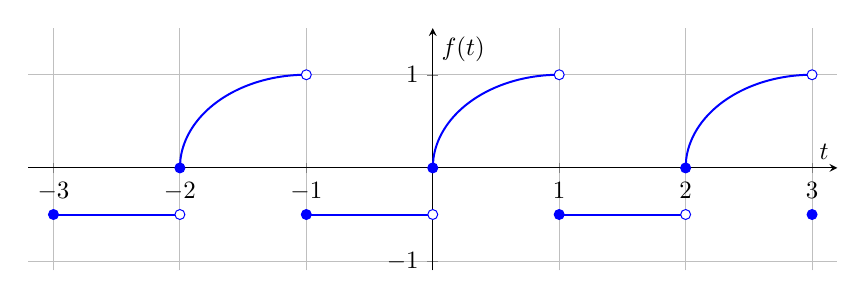
\begin{tikzpicture}[scale=.9]
		\begin{axis}[
			axis lines=middle,
			xmin=-3.2, xmax=3.2,
			ymin=-1.1, ymax=1.5,
			xtick={-3, -2,-1,0,1,2,3},
			ytick={-1,0,1},
			xlabel={$t$},
			ylabel={$f(t)$},
			grid=both,
			width=13cm,
			height=5cm,
			samples=200,
			domain=0:6,
			]
			
			% Semicircular arcs: f(x) = sqrt(1 - (x - shift)^2)
			\addplot[blue, thick, domain=-3:-2]   {-0.5};
			\addplot[blue, thick, domain=-2:-1]   {sqrt(1 - (x +1)^2)};
			\addplot[blue, thick, domain=-1:0]   {-0.5};
			\addplot[blue, thick, domain=0:1]   {sqrt(1 - (x - 1)^2)};
			\addplot[blue, thick, domain=1:2]   {-0.5};
			\addplot[blue, thick, domain=2:3]   {sqrt(1 - (x - 3)^2)};
		
			%\node at (axis cs:1,1.1) {$f(x)$};
			
			% Dots to indicate discontinuities
			\foreach \x in {-2,0,2,4}
			\addplot[only marks, mark=*, blue] coordinates {(\x,0)};
			
			\foreach \x in {-2,0,2,4}
			\addplot[only marks, mark=*, fill=white, draw=blue]  coordinates {(\x,-0.5)};
			
				\foreach \x in {-3,-1,1,3}
			\addplot[only marks, mark=*, blue] coordinates {(\x,-0.5)};
			
			\foreach \x in {-1,1,3}
			\addplot[only marks, mark=*, fill=white, draw=blue]  coordinates {(\x,1)};
			
		\end{axis}
	\end{tikzpicture}
	\caption{A piecewise continuous periodic function $f(t)$ with period $T = 2$.}
	\label{fig:piecewise-periodic}
	\end{figure}
A piecewise continuous periodic function $f(t)$ with a period $T$  has the following property:
\[f(t) = f(t+T)  = f(t+2T) = \cdots = f(t+nT)\] 
%and
%\[f(t) = f(t-T)  = f(t-2T) = \cdots = f(t-nT),\] 
 for all positive integers $n.$  This property is visualized in Figure~\ref{fig:piecewise-periodic}. 
 To compute $\mathscr{L}\{f(t)\},$ we express it as an infinite series of integrals as follows:
 \[\begin{split}
 	\mathscr{L}\{f(t)\}& =\int_0^\infty f(t) e^{-st}\, dt\\
 	&= \int_0^T f(t) e^{-st}\, dt+ \int_T^{2T} f(t) e^{-st}\, dt+ \int_{2T}^{3T} f(t) e^{-st}\, dt +\dots\\
 	&=\int_0^T f(t) e^{-st}\, dt + \int_0^T f(t+T) e^{-s(t+T)}\, dt\\
 	& \quad + \int_0^T f(t+2T) e^{-s(t+2T)}\, dt+ \dots+ \int_0^T f(t+nT) e^{-s(t+nT)}\, dt+\cdots\\
 	&=\int_0^T f(t) e^{-st}\, dt\;\Big(1+e^{-sT}+ e^{-2sT} + \dots+ e^{-nsT}+\cdots \Big)\\
 	&=\int_0^T f(t) e^{-st}\, dt\;\; \sum_{n=0}^\infty e^{-nsT}.
 \end{split}
 \]
 Since the geometric series \(\ds \sum_{n=0}^\infty e^{-nsT}\) converges for $s>0$ to \(\ds \frac{1}{1- e^{-sT}},\)
  we obtain
  \begin{equation}\label{Laplace-periodic-function}
  	\boxed{\mathscr{L}\{f(t)\} = \frac{1}{1- e^{-sT}}\int_0^T f(t) e^{-st}\, dt.}
  \end{equation}
 
\begin{example}
	Let us revisit $\mathscr{L}\{\sin(kt)\}.$ Using (\ref{Laplace-periodic-function}) with $T= 2\pi/k$, we obtain
\[	\mathscr{L}\{\sin(kt)\} = \frac{1}{1- e^{-2\pi s/k}}\int_0^{2\pi/k} \sin(kt) e^{-st}\, dt.\]
We compute 
\[\int_0^{2\pi/k} \sin(kt) e^{-st}\, dt=\frac{k}{s^2+k^2}\left( 1- e^{-2\pi s/k}\right).\]
Hence \[ \mathscr{L}\{\sin(kt)\} =\frac{k}{s^2+k^2},\]
as expected.
\end{example}
The example above suggests that  the direct computation of the Laplace transform of a periodic function may  be more convenient.

The example below concerns a periodic function acting as the source term of an initial value problem.

\begin{example}
	Consider the initial value problem $y'+ y = f(t), \; y(0) = 0,$ where $f(t)$ is given by
	\[f(t) = \begin{cases}
		1 &\text{if } 0\le  t\le 1,\\
		0 &\text{if } 1< t < 2,
	\end{cases}\]
	 and $f(t) = f(t+2)$ for all $t$ in $(-\infty, \infty).$ 
	 The graph of $f$ on $[0, \infty)$ is shown below.
	 
%\textcolor{ red}{Open this later}
	 \begin{center}
	 	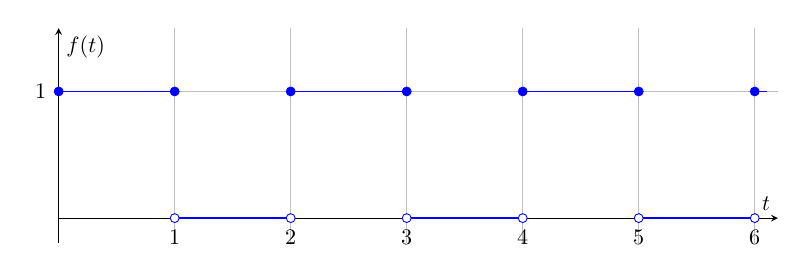
\begin{tikzpicture}[scale=.8]
	 			\begin{axis}[
	 					axis lines=middle,
	 					xmin=0, xmax=6.2,
	 					ymin=-0.2, ymax=1.5,
	 					xtick={0,1,2,3,4,5,6},
	 					ytick={0,1},
	 					xlabel={$t$},
	 					ylabel={$f(t)$},
	 					grid=both,
	 					width=13cm,
	 					height=5cm,
	 					samples=100,
	 					domain=0:6,
	 					]
	 					
	 					% Square wave segments (period 2: [0,1)=1, [1,2)=-1, repeat)
	 					\addplot[blue, thick, domain=0:1]   {1};
	 					\addplot[blue, thick, domain=1:2]   {0};
	 					\addplot[blue, thick, domain=2:3]   {1};
	 					\addplot[blue, thick, domain=3:4]   {0};
	 					\addplot[blue, thick, domain=4:5]   {1};
	 					\addplot[blue, thick, domain=5:6]   {0};
	 					\addplot[blue, thick, domain=6:6.1] {1};
	 					
	 					% Dots to indicate discontinuities
	 					\foreach \x in {0,1,2,3,4,5,6}
	 					\addplot[only marks, mark=*, blue] coordinates {(\x,1)};
	 					\foreach \x in {1,2,3,4, 5,6}
	 					\addplot[only marks, mark=*, fill=white, draw=blue] coordinates {(\x,0)};
	 				\end{axis}
	 		\end{tikzpicture}
	 \end{center}
	 Then 
	 \[\begin{split}
	 	F(s) &= \frac{1}{1-e^{-2s}}\int_0^2 f(t) e^{-st}\, dt\\
	 	 &= \frac{1}{1-e^{-2s}}\int_0^1 e^{-st}\, dt\\
	 	 &  = \frac{1}{1-e^{-2s}}\left(\frac{e^{-s}-1}{-s}\right)\\
	 	 &= \frac{1}{s(1+e^{-s})}.
	 	\end{split}
	 	\]
	 	Taking the Laplace transform of the differential equation, we get
	 	\[sY(s) - y(0) + Y(s) = F(s).\] With $y(0) = 0,$ we have
	 	\[Y(s) = \frac{1}{s(s+1)(1+e^{-s})}.\]
	 	Since \[\ds \frac{1}{s(s+1)} = \frac{1}{s}- \frac{1}{s+1}\] and \[\ds\frac{1}{1+e^{-s}} = \sum_{n=0}^\infty (-1)^ne^{-ns},\] it follows that 
	 	\[Y(s) = \left(\frac{1}{s}- \frac{1}{s+1}\right)\sum_{n=0}^\infty (-1)^ne^{-ns}.\]
	In view of the shifting on the $t-$axis property discussed in Example~\ref{shiting-on-t-axis},  the solution $y(t)$ of the initial value problem is
	 	\[y(t)  =  \sum_{n=0}^{\infty}(-1)^n \mathcal{U}(t-n)\; (1- e^{-(t-n)}).\]
	% \textcolor{red}{Open this figure later}
	\begin{figure}[!htb]
		\centering
	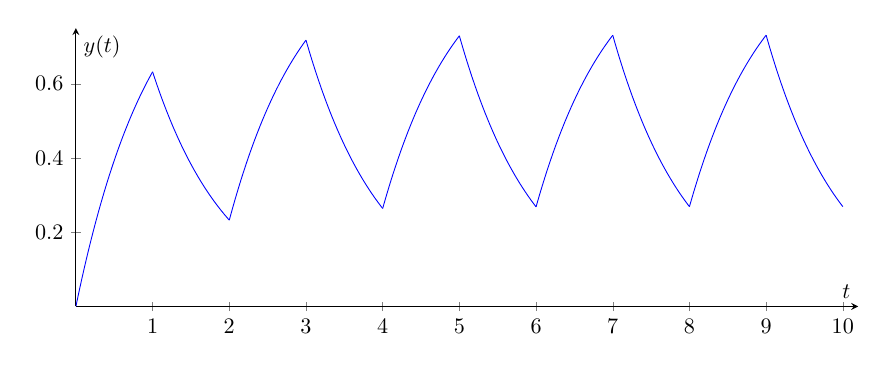
\begin{tikzpicture}[scale=0.8]
		\begin{axis}[
			axis lines=middle,
			xmin=0, xmax=10.2,
			ymin=0, ymax=0.75,
			samples=500,
			domain=0:10,
			%grid=both,
			width=14cm,
			height=6cm,
			xlabel={$t$},
			ylabel={$y(t)$}
			]
			
		 \addplot[blue, domain=0:1]     {1 - exp(-x)};
		 \addplot[blue, domain=1:2]     {1 - exp(-x) - (1 - exp(-(x - 1)))};
		 \addplot[blue, domain=2:3]     {1 - exp(-x) - (1 - exp(-(x - 1))) + (1 - exp(-(x - 2)))};
		 \addplot[blue, domain=3:4]     {1 - exp(-x) - (1 - exp(-(x - 1))) + (1 - exp(-(x - 2))) - (1 - exp(-(x - 3)))};
		 \addplot[blue, domain=4:5]     {1 - exp(-x) - (1 - exp(-(x - 1))) + (1 - exp(-(x - 2))) - (1 - exp(-(x - 3))) + (1 - exp(-(x - 4)))};
		 \addplot[blue, domain=5:6]     {1 - exp(-x) - (1 - exp(-(x - 1))) + (1 - exp(-(x - 2))) - (1 - exp(-(x - 3))) + (1 - exp(-(x - 4))) - (1 - exp(-(x - 5)))};
		 \addplot[blue, domain=6:7]     {1 - exp(-x) - (1 - exp(-(x - 1))) + (1 - exp(-(x - 2))) - (1 - exp(-(x - 3))) + (1 - exp(-(x - 4))) - (1 - exp(-(x - 5))) + (1 - exp(-(x - 6)))};
		 \addplot[blue, domain=7:8]     {1 - exp(-x) - (1 - exp(-(x - 1))) + (1 - exp(-(x - 2))) - (1 - exp(-(x - 3))) + (1 - exp(-(x - 4))) - (1 - exp(-(x - 5))) + (1 - exp(-(x - 6))) - (1 - exp(-(x - 7)))};
		 \addplot[blue, domain=8:9]     {1 - exp(-x) - (1 - exp(-(x - 1))) + (1 - exp(-(x - 2))) - (1 - exp(-(x - 3))) + (1 - exp(-(x - 4))) - (1 - exp(-(x - 5))) + (1 - exp(-(x - 6))) - (1 - exp(-(x - 7))) + (1 - exp(-(x - 8)))};
		 \addplot[blue, domain=9:10]    {1 - exp(-x) - (1 - exp(-(x - 1))) + (1 - exp(-(x - 2))) - (1 - exp(-(x - 3))) + (1 - exp(-(x - 4))) - (1 - exp(-(x - 5))) + (1 - exp(-(x - 6))) - (1 - exp(-(x - 7))) + (1 - exp(-(x - 8))) - (1 - exp(-(x - 9)))};
  \end{axis}
\end{tikzpicture}
\caption{Graph of $\ds f(t) = \sum_{n=0}^{10} (-1)^n \mathcal{U}(t - n)\; (1 - e^{n - t}) $}
\end{figure}


%Do not open the following figure unless reviewed
%	\begin{figure}
%		\centering
%		\includegraphics[width=0.7\linewidth]{chap05/figures/periodic-source}
%		\caption{}
%		\label{fig:periodic-source}
%	\end{figure}
	 	
\end{example} 


\begin{Exercise}\label{EX74}
	\vspace{-\baselineskip}% <-- You don't need this line of code if there's some text here
	\Question\label{6-4-1} Sketch the graph of three periods of each function below and compute its Laplace transform. The interval for the first period is provided.
	\begin{tasks}[resume=false](2)
		\task \label{6-4-1(i)} $f(t) = \cos t, \quad 0\le t < \pi$
		\task\label{6-4-1(ii)} $f(t) =  t, \quad 0\le t < 3$
		\task\label{6-4-1(iii)} $f(t) =t-2, \quad 0\le t  < 4$
		\task\label{6-4-1(iv)} $f(t) = \begin{cases}
			1	& \text{if } 0\le t< 1\\
			-1 		& \text{if } 1\le  t< 2\\
		\end{cases}$
		
		\task\label{6-4-1(v)} $f(t) = \begin{cases}
			\sin t 	& \text{if } 0\le t< \pi\\
			0 		& \text{if } \pi\le  t< 2\pi\\
		\end{cases}$
		\task\label{6-4-1(vi)} \(f(t) = \begin{cases}
		e^{-t}\sin t 	& \text{if } 0\le t< \pi\\
		0 		& \text{if } \pi\le  t< 2\pi\\
	\end{cases}\)
	\end{tasks}
	
	
	\Question Solve the following initial value problems using the Laplace transform method. You will need $\frac{1}{1-x} = \sum_{n=0}^\infty (-1)^n x^n$ and $\frac{1}{1+x} = \sum_{n=0}^\infty  x^n$  when $|x| <1.$
	\begin{tasks}[resume=false](1)
		\task $y''+4y'+3y = f(t), \quad y(0) = 0, y'(0) = 0$ where \(f(t) =\begin{cases}
			0 &\text{if } 0\le  t\le 1\\
			1 &\text{if } 1< t < 2 
		\end{cases}\)
		 and $f(t) = f(t+2)$ for all $t$ in $(-\infty, \infty).$ 
	\task $y''+4y'+4y = f(t),\quad y(0) = 0, y'(0) = 0,$ where 
	\(f(t)\) is the periodic function in part \ref{6-4-1(iv)} of Problem~\ref{6-4-1}.
	\task $y''+3y'+2y = f(t),\quad y(0) = 0, y'(0) = 0,$ where 
	\(f(t)\) is the periodic function in part \ref{6-4-1(v)} of Problem~\ref{6-4-1}.
		\task $y''+4y = f(t),\quad y(0) = 0, y'(0) = 0,$ where 
	\(f(t)\) is the periodic function in part \ref{6-4-1(ii)} of Problem~\ref{6-4-1}.	
	\end{tasks}
	
\end{Exercise}

\setboolean{firstanswerofthechapter}{true}
\begin{multicols}{2} \scriptsize
	\begin{Answer}[ref={EX74}]
		\Question 
		\begin{tasks} 
			\task 	\includegraphics[width=0.9\linewidth]{chap05/Mathematica/7-4-1}\newline
			$\frac{s\left(1+e^{-\pi  s}\right)}{\left(s^2+1\right)\left(1-e^{-\pi  s}\right) }$
			\task \includegraphics[width=0.9\linewidth]{chap05/Mathematica/7-4-2}\newline
			$\frac{1-e^{-3 s} (3 s+1)}{\left(1-e^{-3 s}\right) s^2}$
			\task \includegraphics[width=0.9\linewidth]{chap05/Mathematica/7-4-3}\newline
			$\frac{1-2 s-e^{-4 s} (2 s+1)}{\left(1-e^{-4 s}\right) s^2}$
			\task \includegraphics[width=0.9\linewidth]{chap05/Mathematica/7-4-4}\newline
			$\frac{1-e^{-s}}{\left(1-e^{-2 s}\right) s}$
			\task \includegraphics[width=0.9\linewidth]{chap05/Mathematica/7-4-5}\newline
			$\frac{e^{-\pi  s}+1}{\left(1-e^{-2 \pi  s}\right) \left(s^2+1\right)}$
			\task \includegraphics[width=0.9\linewidth]{chap05/Mathematica/7-4-6}\newline
			$\frac{e^{-\pi  s}+1}{\left(1-e^{-2 \pi  s}\right) \left(s^2+1\right)}$
		\end{tasks} 
		\Question 
		\begin{tasks}[resume=false]
			\task $F(s) = \frac{e^{-s}}{s(1+e^{-s})} = -\frac{1}{s}+\frac{1}{s(1-e^{-s})}$,\\ $Y(s) = \frac{F(s)}{(s+1)(s+3)}\\= \left(\frac{1}{3 s}-\frac{1}{2 (s+1)}+\frac{1}{6 (s+3)}\right)\ds\sum_{n=1}^\infty (-1)^{n} e^{-ns}$;
			$y(t) =\sum_{n=1}^\infty (-1)^{n} \mathcal{U}(t-n) \\\left(\frac13- \frac{1}{2}e^{-(t-n)} +\frac{1}{6}e^{-3(t-n)}\right).$
			\task $F(s) = -\frac{1}{s}+\frac{2}{s(1+e^{-s})}$,\\ $Y(s) = \frac{F(s)}{(s+2)^2}\\= -\frac{1}{s(s+2)^2}+ \frac{2}{s(s+2)^2}\sum_{n=0}^\infty (-1)^{n} e^{-ns}$\\
			$= \frac{1}{4 (s+2)}+\frac{1}{2 (s+2)^2}-\frac{1}{4 s}\\+\left(\frac{1}{2 s}-\frac{1}{2 (s+2)}-\frac{1}{(s+2)^2}\right)\ds\sum_{n=0}^\infty (-1)^{n} e^{-ns}$;\\
			$y(t) = \frac{1}{2} e^{-2 t} t+\frac{e^{-2 t}}{4}-\frac{1}{4}\\ + \ds\sum_{n=0}^\infty (-1)^{n} \mathcal{U}(t-n) \big(\frac{1}{2}-\frac{e^{-2 (t-n)}}{2}\\-e^{-2 (t-n)} (t-n)\big)$
			
			\task $F(s) = \frac{1}{(1-e^{-\pi  s})(s^2+1)}$; \\$Y(s) = \frac{F(s)}{(s+1)(s+2)}\\ =\frac{1}{(1-e^{-\pi  s})(s^2+1)(s+1)(s+2)} $\\$=\ds\frac{1}{(s^2+1)(s+1)(s+2)}\sum_{n=0}^\infty e^{-n\pi s} $;
			$y(t) = \frac{1}{10}\sum_{n=0}^\infty \mathcal{U}(t- n\pi)\\ \big( 5e^{-(t-n\pi)}- 2 e^{-2(t-n\pi)}\\
			-3 \cos(t-n\pi)+\sin (t-n\pi)\big)$
			\task $F(s) = \frac{1}{s^2}+\frac{3}{s}-\frac{3}{s(1-e^{-3s})}$;  $Y(s)  = \frac{1}{s^2(s^2+4)}+\frac{3}{s(s^2+4)}-\frac{3}{s (s^2+4)(1-e^{-3s})} =\frac{1}{s^2(s^2+4)} -\frac{3}{s(s^2+4)}\ds\sum_{n=1}^\infty  e^{-3ns}\\
			=\frac{1}{4}\left(\frac{1}{s^2} - \frac{1}{s^2+4}\right)\\ -\frac{3}{4}\left(\frac{1}{s}-\frac{s}{s^2+4}\right)\ds\sum_{n=1}^\infty  e^{-3ns}$;\\
			$ y(t) = \frac{1}{4} ( t- \sin t \cos t)\\- \frac{3}{2} \ds\sum_{n=1}^\infty \mathcal{U}(t-3n) \sin^2(t-3n)$
		\end{tasks} 
	\end{Answer}
\end{multicols}
\setboolean{firstanswerofthechapter}{false}

\section{A Convolution Theorem}
A crucial step in solving a linear initial value problem using Laplace transforms is determining the inverse Laplace transform of the solution's Laplace transform. This step can become challenging when the expression, whose inverse Laplace transform is desired, is complicated. In this section, we discuss a procedure with which we can determine the inverse Laplace transform of an expression that is  a product of  known Laplace  transforms. For example, we recall that \[\mathscr{L}^{-1}\left\{\ds\frac{1}{s^2}\right\} = t \quad \text{ and }\quad  \mathscr{L}^{-1}\left\{\ds\frac{2}{s^3}\right\} = t^2.\]
However, if we were to compute   
\[ \mathscr{L}^{-1}\left\{\ds\left(\frac{1}{s^2}\right) \left(\frac{2}{s^3}\right)\right\},\] a direct way is to see this problem as
\[ \mathscr{L}^{-1}\left\{\frac{2}{s^5}\right\} = \frac{2}{4!}\; t^4 = \frac{t^4}{12}.\]
This leads to a natural question: in what way can we combine $t$ and $t^2$ to produce $t^4/12$? The  operation for combining inverse Laplace transforms—specifically, to determine the inverse of a product—is known as \textit{convolution}, which is formalized in the following definition.

\begin{definition}\label{def:convolution}
	Let $f$ and $g$ be functions on $[0, \infty).$ The \textbf{\textit{convolution}} of $f$ and $g$, denoted by $f\ast g$, is the function defined by
	\[(f\ast g)(t) = \int_0^t f(u) g(t-u)\, du\] whenever the integral exists for a given $t$ in $[0, \infty).$
\end{definition}
For computational purposes, $(f * g)(t)$ may also be written as $f(t) * g(t)$.
It can be proved that $f\ast g = g\ast f;$ see, for example, \ref{7-5-2}\;\ref{7-5-2(i)} in  \textbf{Exercises~\ref{EX75}}. The convolution $1\ast f$ is particularly useful, and it  is given by
\begin{equation}\label{special-convolution}
	(1\ast f)(t) = \int_0^t f(u) \, du.
	\end{equation}
	See, also,  \ref{7-5-2}\;\ref{7-5-2(v)} in \textbf{Exercises~\ref{EX75}}.
\begin{example}
Let us return to the example discussed before Definition~\ref{def:convolution}  and calculate the convolution of $f(t) =t$ and $g(t) =t^2$. We have
	\[
	\begin{split}
		(f\ast g)(t)& = \int_0^t u (t-u)^2\, du\\
		&= \int_0^t (t^2u-2tu^2 +u^3)\, du\\
		&= \left[t^2\frac{u^2}{2}-2t\frac{u^3}{3}+\frac{u^4}{4}\right]_0^t\\
		&=\frac{t^4}{2}-\frac{2t^4}{3}+\frac{t^4}{4}\\
		&=\frac{t^4}{12},
	\end{split}
	\]
as expected.\hfill$\clubsuit$
\end{example}
We now state the most important theorem of this section. 
\begin{theorem}[Convolution Theorem]\label{thm:convolution-theorem}
	Let $f$ and $g$ be piecewise continuous functions on $[0,\infty)$ and of the exponential order $\alpha$ as $t\to\infty$.
	Then
	\[ \mathscr{L}\{(f\ast g)(t)\}= F(s) \,G(s);\]
	or equivalently,
	\[\mathscr{L}^{-1}\left\{ F(s) G(s)\right\} =\mathscr{L}^{-1}\{F(s)\}\ast \mathscr{L}^{-1}\{G(s)\}\] for $s>\alpha.$
\end{theorem}

To see how this theorem holds, we need to use a method for changing the order of an iterated integral. 
%See  Appendix~\ref{Leibniz-Rule} for further details. 
We include a proof of the Convolution Theorem below for the sake of completeness; however, not to be distracted from the proof, the reader may choose to skip it for now and proceed directly to apply the theorem.

\begin{proof}[Proof of Theorem~\ref{thm:convolution-theorem}]
We recall that 
\[
	F(s)  = \int_0^\infty e^{-s\eta} f(\eta) \, d\eta\quad \text{ and }\quad 
	G(s) = \int_0^\infty e^{-su} g(u) \, du.\] Then 
\begin{align*}
		F(s) G(s) & = \int_0^\infty e^{-s\eta} f(\eta) \, d\eta\; \int_0^\infty e^{-su} g(u) \, du\\
		&=\int_0^\infty g(u) \left( \int_0^\infty e^{-s(\eta+u)} f(\eta) \, d\eta \right) \, du\\
		& = \int_0^\infty g(u) \left( \int_u^\infty e^{-st} f(t - u) \, d\xi \right) \, du,
\end{align*}
where $t=\eta+u.$
By changing the order of integration, we obtain
\begin{align*} F(s) G(s)&=\int_0^\infty e^{-s t} \left( \int_0^t g(u)  f(t - u) \, du \right) \, dt \\
	&=\int_0^\infty e^{-st} (g\ast f)(t)\, dt\\
	& = \mathscr{L}\{(f\ast g)(t)\}.\qedhere
\end{align*}
\end{proof}
Some fundamental properties of the convolution operation are discussed in  Exercises~\ref{EX75}; see the problem~\ref{7-5-2}.

The following theorem concerns an interesting application of Theorem~\ref{thm:convolution-theorem} to linear initial value problems that involve the Dirac delta functions.  


\begin{theorem}\label{thm:IVP-convolution}
	Let $y_\delta(t)$ denote the solution of the initial value problem
 \begin{equation}\label{IVP-delta1}
	ay''+by'+cy = \delta(t), \quad y(0) = 0, y'(0) = 0.
\end{equation}
The the solution $y(t)$ of the initial value problem 
\begin{equation}\label{IVP-delta2}
	ay''+by'+cy = g(t), \quad y(0) = 0, y'(0) = 0
	\end{equation} where $a, b, c$ are constants with $a\ne 0,$ and $g$ is a piecewise continuous function that is of exponential order as $t\to\infty,$ is given by
	\[y(t) = (y_\delta \ast g)(t).\]
\end{theorem}

We first remark that $y'$ and $y''$ in (\ref{IVP-delta1}) are to be interpreted  differently (as \textit{distributional derivatives}) because of the presence of $\delta(t)$ on the right side of the equation. The fact beyond the scope of this book is that the Laplace transforms of  distributional derivatives coincide with the Laplace transforms of the classical derivatives.  


\begin{proof}
	Applying the Laplace transform $\L$ to the initial value problem (\ref{IVP-delta1}) and using $y(0)= y'(0)=0$  yields
	\[(as^2+bs +c)Y(s)= 1,\]that is,
	\[Y(s)= \frac{1}{as^2+bs +c}.\] Then 
	\[y_\delta(t) = \L^{-1}\left\{\frac{1}{as^2+bs +c}\right\}.\]
	
Now, taking the Laplace transform $\L$ of the initial value problem (\ref{IVP-delta2}) and using $y(0)= y'(0)=0$  yields
	\[(as^2+bs +c)Y(s)= G(s),\]that is,
	\[Y(s)= \frac{1}{as^2+bs +c}\; G(s).\] By Theorem~\ref{thm:convolution-theorem}, we obtain
	\[y(t) = \L^{-1}\left\{\frac{1}{as^2+bs +c}\right\}\ast \L^{-1}G(s) = y_\delta(t) \ast g(t).\qedhere\] 
\end{proof}
\begin{example}
	Consider the initial value problem $y''+ y= e^t,\; y(0) = y'(0)= 0.$
\end{example}
\begin{solution} In the context of Theorem~\ref{thm:IVP-convolution}, the solution to the initial value problem $y''+ y= \delta (t),\; y(0) = 0, \, y'(0)= 0,$ is given by 
	\[ y_\delta(t) = \L^{-1}\left\{\frac{1}{s^2+1}\right\} = \sin t.\]  We note here that $y'_\delta(t) =\cos t,$ and
	$y'_\delta (0+) = 1,$ which reflects  the behavior of $\delta(t)$ at $t = 0$ because  $y'_\delta $ would then have a jump discontinuity at $t = 0$, so that $y''_\delta $ would  be the Dirac delta $\delta(t)$ as a distribution.\footnote[1]{In the distribution theory, the distributional derivative of $\mathcal U(t)$ is the Dirac delta $\delta(t)$.} By Theorem~\ref{thm:IVP-convolution}, the solution to the given initial value problem is 
	\[ y(t) = y_\delta(t) \ast e^t = \sin t \ast e^t = -\frac{1}{2}\left(-e^t+\sin t+\cos t\right)\]
on $(-\infty, \infty).$
\end{solution}


\begin{Exercise}\label{EX75}
	\vspace{-\baselineskip}% <-- You don't need this line of code if there's some text here
	
	\Question\label{7-5-1}
For the functions $f$ and $g$ on $[0, \infty)$ given below, compute $f\ast g$, $\L\{(f\ast g)(t) \}$ and verify that $\L\{(f\ast g)(t) \} =\L\{f(t)\}\, \L\{g(t)\}.$
	
	\begin{tasks}(1)
		\task $ f(t) = g(t) = 1$ 
		\task $ f(t) = g(t) = e^{kt},$ where $k$ is any constant   
		\task $ f(t) = \sin t,\; g(t) = e^{kt},$ where $k$ is any real number
		\task $ f(t)= g(t) = \sin (\omega t),$ where $\omega$ is any real number
		\task $ f(t)= \sin(\omega t),\; g(t) = \cos(\omega t),$ where $\omega$ is any real number
	\end{tasks}
	
	\Question \label{7-5-2}
	Let $f, g, h$ be functions defined on the interval $[0, \infty)$, and assume that all the convolutions below are well-defined. Use the definition of the convolution  to prove the following properties.
		\begin{tasks}(1)
				\task\label{7-5-2(i)} $f\ast g= g\ast f$   
				\task $f\ast (g\ast h) = (f\ast g) \ast h$ 
				\task $f \ast (g+h)= f\ast g+ f\ast h$ 
				\task $f\ast k g= k( f\ast g),$ where $k$ is any constant
				\task\label{7-5-2(v)} $1\ast f(t) = \int_0^t f(u) \, du$
			\end{tasks}
	
	
	\Question \label{7-5-3}
	Use the convolution theorem (Theorem~\ref{thm:convolution-theorem}) to find the Laplace transform of  each of the following functions. Also,   find the convolution in  each one of \ref{7-5-3(i)}--\ref{7-5-3(v)}.

	\begin{tasks}(2)
		\task\label{7-5-3(i)}  $1\ast t\ast  t^2$
		\task $1\ast t^2\ast \sin t$
		\task  $1\ast \cos t\ast \sin t$
		\task $1\ast \sin t\ast \mathcal{U} (t-2)$ 
		\task\label{7-5-3(v)} $1\ast \mathcal{U} (t-2)\ast \mathcal{U} (t-5)$ 
		\task $\ds\int_0^t e^u\, du$
		\task $\ds\int_0^t \sin u\, du$
		\task $\ds\int_0^t u\sin u\, du$
		\task $\ds\int_0^t \sin u\,\cos(t-u)\, du$
		\task $\ds t\int_0^t \sin u\,\cos(t-u)\, du$
		
	\end{tasks}
\Question \label{7-5-4}
	Use the convolution theorem (Theorem~\ref{thm:convolution-theorem}) to find each of the following inverse Laplace transforms.
	\begin{tasks}[resume=false](2)
		\task $\ds\mathscr{L}^{-1}\left\{\frac{1}{(s+1)(s-1)}\right\}$
		\task $\ds\mathscr{L}^{-1}\left\{\frac{1}{s^3(s-1)}\right\}$
		\task $\ds\mathscr{L}^{-1}\left\{\frac{2}{(s^2+4)^2}\right\}$
		\task $\ds\mathscr{L}^{-1}\left\{\frac{s^2}{(s^2+4)^2}\right\}$
		\task $\ds\mathscr{L}^{-1}\left\{\frac{s^2}{(s^2-4)^2}\right\}$
		\task $\ds\mathscr{L}^{-1}\left\{\frac{1}{s^2(s^2+4)^2}\right\}$
	\end{tasks}

\Question \label{7-5-5} Solve the following integral or integro-differential equations using the Laplace transform.
\begin{tasks}[resume=false](1)
	\task $\ds y(t)+\int_0^t y(u)\, du = 1$
	\task $\ds y(t) = te^t+ \int_0^t u\,y(t-u)\, du$
	\task $\ds y'(t) = 1-\cos t - \int_0^t y(u)\, du, \quad y(0) =0$
	\task $\ds y'(t) +4 y(t) + 4 \int_0^t y(u)\, du=1, \quad y(0) =0$
\end{tasks}

\Question\label{7-5-6} Use Theorem~\ref{thm:IVP-convolution} to solve the following initial value problems.
\begin{tasks}[resume=false](1)
	\task $y'-3y= \sin t, \quad y(0)= 0$
	\task $y''+y= \sin t, \quad y(0)= 0, \; y'(0)=0$
	\task $y''+4y'+3y= e^t, \quad y(0)= 0, \; y'(0)=0$
	\task $y''+4y'+13y= \cos t, \quad y(0)= 0, \; y'(0)=0$
\end{tasks}
	
\Question \label{7-5-7} Let $f$ be a continuous function defined on the interval $[0, \infty)$, and assume that all the convolutions below are well-defined. Show the following properties of the convolution operation.
	\begin{tasks}(1)
		\task $f\ast \delta = f.$ (This means that $\delta$ is an identity element for the convolution operation.)
		\task $f(t)\ast \delta (t-a) =  \mathcal{U}(t-a) f(t-a),$ where $a\ge 0$ and is a fixed real number. 
	\end{tasks}	
	
\Question \label{7-5-8} 	Let $f, g$ be  functions with continuous derivatives  on the interval $[0, \infty)$ and of exponential order as $t\to\infty$.  Assume further that all the convolutions below are well-defined. Use the convolution theorem (Theorem~\ref{thm:convolution-theorem}) to prove the following properties.
	\begin{tasks}(1)
		\task $1\ast f'(t) = f(t) - f(0).$
		\task $(f\ast g)'(t) = g(0) f(t) + (g'\ast f)(t) = f(0) g(t) + (g\ast f')(t).$
	\end{tasks}	
The above properties are also valid for any differentiable functions $f$ and $g$, not necessarily of exponential order as $t\to\infty$, in light of the Leibniz rule\footnote{\scriptsize\begin{equation}\label{Leibniz-rule}
		\frac{d}{dt}\int_{a(t)}^{b(t)} f(u, t) \, du  = f(b(t), t) \frac{db(t)}{dt} - f(a(t), t)\frac{da(t)}{dt} +\int_{a(t)}^{b(t)} \frac{\partial f}{\partial t} (u, t)\, du
		\end{equation} } for differentiating an integral (see Theorem~\ref{thm:DUI-v2} in Appendix~\ref{Leibnitz Rule-Improper Integrals}).
	
	
	
\Question \label{7-5-9} By using the Leibniz rule (\ref{Leibniz-rule}), convert each of the following integral or integro-differential equations into an equivalent initial value problem and then solve it by using your favorite method. Compare your answers to those obtained in Problem~\ref{7-5-5}.
\begin{tasks}[resume=false](1)
	\task $\ds y(t)+\int_0^t y(u)\, du = 1$
	\task $\ds y(t) = te^t+ \int_0^t u\,y(t-u)\, du$
	\task $\ds y'(t) = 1-\cos t - \int_0^t y(u)\, du, \quad y(0) =0$
	\task $\ds y'(t) +4 y(t) + 4 \int_0^t y(u)\, du=1, \quad y(0) =0$
\end{tasks}


\Question\label{7-5-10} Solve the following initial value problems using the Laplace transform. Also, determine whether the solutions are continuous at the point(s) of concentration of the involved Dirac delta functions(s).
\begin{tasks}[resume=false](1)
	\task $y'-3y= \delta(t-1), \quad y(0)= 0$
	\task $y'+4y= \delta(t-2), \quad y(0)= 1$
	\task $y''+4y= \delta(t-2\pi), \quad y(0)= 0, \; y'(0)=0$
	\task $y''+4y'+3y= \delta(t-2\pi), \quad y(0)= 0, \; y'(0)=0$
	\task $y''+4y'+13y= \delta(t-2\pi), \quad y(0)= 0, \; y'(0)=0$
	\task $y''+4y'+3y= \delta(t-2\pi) +\delta(t-3\pi), \quad y(0)= 0, \; y'(0)=0$
	\task $y''+4y'+13y= \delta(t-2\pi) +\delta(t-3\pi), \quad y(0)= 0, \; y'(0)=0$
\end{tasks}

%\Question A 1 lb mass is suspended from the lower end of a vertical spring, stretching the spring 4 feet to reach its equilibrium position. The mass is then pulled downward an additional 1 foot and released from rest. Suppose that no damping and no external forces act on the system.   Let $y(t)$ denote the displacement of the mass at time $t$, with the convention that displacements measured downward from the equilibrium position are  positive. 
%\begin{enumerate}[label = (\roman*)]
%	\item Write down the initial value problem for the displacement $y(t).$
%	\item Find the first time at which the mass passes through the equilibrium position heading upward.
%	\item Determine the Dirac delta function  that models the impulsive force with which the mass must be struck with a hammer at the first upward passage through the equilibrium position, in such a way that the mass comes to rest instantly and remains at equilibrium thereafter.
%\end{enumerate}
 
 \Question\label{7-5-11} A 32 lb mass stretches a vertically hanging spring  4 feet to equilibrium. The mass is then pulled down 1 foot and released from rest. Assume no damping or external forces. Let $y(t)$ denote the displacement of the mass from equilibrium at time $t,$ measured positive in the downward direction. (Use $g= 32 ;\text{ft}/\text{s}^2$.)
\begin{enumerate}[label =(\roman*)]
	\item Set up an initial value problem for $y(t).$ 
	\item\label{partii} Determine a Dirac delta function that models the impulsive force on the mass exerted by striking it with a hammer to stop it at the first time it passes through equilibrium, keeping it at the equilibrium position thereafter.
	\item Repeat part~\ref{partii} to stop the mass at the second time it passes through equilibrium.
\end{enumerate}

 


\end{Exercise}

\setboolean{firstanswerofthechapter}{true}
\begin{multicols}{2}\scriptsize
	\begin{Answer}[ref={EX75}]
		\Question \label{7-5-1a}
		\begin{tasks}
			\task $t,\quad \frac{1}{s^2}$
			\task $t  e^{k t},\frac{1}{(k-s)^2}$
			\task $\frac{e^{k t}-k \sin t-\cos t}{k^2+1},\quad \frac{1}{\left(s^2+1\right) (s-k)}$
			\task $\frac{ \sin (\omega t )-\omega t \cos (\omega t )}{2 \omega },\frac{\omega ^2}{\left(s^2+\omega ^2\right)^2}$
			\task $\frac{1}{2} t \sin (\omega t),\frac{s \omega }{\left(s^2+\omega ^2\right)^2}$
		\end{tasks} 
		
	\Question\label{7-5-2a} Left as an exercise.
	
	\Question \label{7-5-3a}
	\begin{tasks}(1)
		\task $\frac{2}{s^6},\quad \frac{t^5}{60}$
		\task $\frac{1}{3} \left(\frac{6}{s^4}-\frac{6}{s^2}+\frac{6}{s^2+1}\right),\\ \frac{1}{3} \left(t^3-6 t+6 \sin t\right)$
		\task $\frac{1}{2} \left(\frac{1}{s^2+1}-\frac{s^2-1}{\left(s^2+1\right)^2}\right),\\ \frac{1}{2}  (\sin t-t \cos t)$
		\task $\frac{e^{-2 s}}{s^4+s^2},\quad \mathcal{U} (t-2) (t+\sin (2-t)-2)$
		\task $\frac{e^{-6 s}}{s^3},\quad \frac{1}{2} (t-6)^2 \mathcal{U}(t-6)$
		\task $\frac{1}{s(s-1)}$
		\task $\frac{1}{s^3+s}$
		\task $\frac{2}{\left(s^2+1\right)^2}$
		\task $\frac{s}{\left(s^2+1\right)^2}$
		\task $\frac{3 s^2-1}{\left(s^2+1\right)^3}$
	\end{tasks}
			
		\Question\label{7-5-4a}
	\begin{tasks}
		\task  $\frac{1}{2} \left(e^{ t}-e^{-t}\right) =\sinh t$
		\task	$e^t-\frac{t^2}{2}-t-1$
		\task $\frac{1}{8} (\sin (2 t)-2 t \cos (2 t))$
		\task $\frac{1}{4} (\sin (2 t)+2 t \cos (2 t))$
		\task $\frac{1}{8} e^{-2 t} \left(2 t+e^{4 t} (2 t+1)-1\right)$
		\task $\frac{1}{64} (4 t-3 \sin (2 t)+2 t \cos (2 t))$
	\end{tasks}
		
		\Question\label{7-5-5a}
		\begin{tasks}
			\task $y(t) = e^{-t}$
			\task $y(t) = \frac{1}{8}  \left((2 t^2 +3t+1)e^t -e^{-t}\right)$; use the property $f\ast g = g\ast f$	
			\task $y(t)= \frac{1}{2} (\sin t-t \cos t)$
			\task $y(t)=e^{-2 t} t$
		\end{tasks}	
		
			\Question\label{7-5-6a}
		\begin{tasks}
			\task $y(t) = -\frac{1}{10} \theta (t) \left(-e^{3 t}+3 \sin t+\cos t\right).$
			\task $y(t) = \left\{\frac{1}{2} (\sin t-t \cos t)\right\}$
			\task $y(t) = \frac{1}{8} e^{-3 t} \left(e^{2 t}-1\right)^2.$
			\task $\frac{1}{120} \big(3 \sin t+9 \cos t\\-e^{-2 t} (7 \sin (3 t)+9 \cos (3 t))\big)$
		\end{tasks}
		
			
			\Question\label{7-5-7a} 
		\begin{tasks}[resume=false]
			\task $(f\ast \delta)(t) =\int_0^t f(t-u) \delta(u)\,du =f(t)$
			\task $f(t)\ast \delta (t-a) =\int_0^t f(t-u) \delta(u-a)\,du\\
			 =\begin{cases}
			0 , \quad t<a\\
			\int_{-\infty}^\infty f(t-u) \delta(u-a)\, du,\;t\ge a
			\end{cases}\\ = \begin{cases}
			0 , \quad t<a\\
		f(t-a),\; t\ge a
			\end{cases}\\ = \mathcal{U}(t-a) f(t-a).$
		\end{tasks} 
			\Question\label{7-5-8a}
		\begin{tasks}
			\task $\L\{1\ast f'(t)\}= \frac{1}{s} [ s F(s) - f(0)] = F(s) - f(0)/ s.$ Taking $\L^{-1}$ of both sides yields the property.
			\task $\L\{(f\ast g)'(t)\}= s F(s) G(s) - (f\ast g)(0)] = sF(s) G(s) = [sF(s)- f(0)]G(s) + f(0) G(s).$ Taking $\L^{-1}$ of both sides yields the property.
		\end{tasks}
	

	
	\Question\label{7-5-9a} 
	\begin{tasks}[resume=false](1)
		\task Note that $y(0) = 1$.Differentiating with Leibniz rule gives:  $y'(t) +y(t) = 0.$ 
		\task Note that $y(0)=0.$ Differentiating with Leibniz rule gives:  $y'(t) = (t+1)e^t - t y(0) + \int_0^t y(u) \, du.$  Note that $y'(0) = 1.$ Differentiating again gives $y''(t) -y(t) = (t+2) e^t.$
		\task Note that $y'(0)= 0.$ Differentiating yields $y''(t)+y(t) = \sin t$. 
		\task Note that $y'(0)= 1.$ Differentiating gives $y''(t) + 4y'(t)+4 y(t) =0$. 
	\end{tasks}
	
	\Question\label{7-5-10a}
	\begin{tasks}
		\task $y(t) = e^{3 (t-1)} \mathcal{U} (t-1);$ the solution has a jump discontinuity at $t=1.$
		\task $y(t) = e^{-4 t} \left(e^8 \mathcal{U} (t-2)+1\right);$ the solution has a jump discontinuity at $t =2.$
		\task $y(t) = \frac12 \mathcal{U}(t-2\pi) \sin (2t);$ the solution is continuous everywhere including $t= 2\pi$.
		\task $y(t)= \frac{1}{2} e^{2 \pi -3 t} \left(e^{2 t}-e^{4 \pi }\right) \mathcal{U} (t-2 \pi ):$ the solution  is continuous everywhere including $t = 2\pi.$
		\task $y(t) = \frac{1}{3} e^{4 \pi -2 t} \mathcal{U} (t-2 \pi ) \sin (3 t);$ the solution  is continuous everywhere including $t = 2\pi.$
		\task $y(t) = \frac{1}{2}  \left(e^{3\pi-t }-e^{9\pi-3t }\right) \mathcal{U} (t-3 \pi )\\- \frac{1}{2} \left(e^{6 \pi-3t }-e^{2\pi- t}\right) \mathcal{U} (t-2 \pi );$
		the solution  is continuous everywhere including $t = 2\pi, 3\pi.$
		\task $y(t) = \frac{1}{3} e^{2 \pi -2 t} \Big(e^{2 \pi } \mathcal{U} (t-2 \pi )\\-\mathcal{U} (t-\pi )\Big)\sin (3 t);$
			the solution  is continuous everywhere including $t = \pi, 2\pi.$
	\end{tasks}


	\Question\label{7-5-11a}
	\begin{tasks}
	\task $y'' + 4y =0, \quad y(0) = 1, y'(0) =0.$
	\task $y'' + 4y =2 \delta(t- \pi/4), \quad y(0) = 1, y'(0) =0$; $y(t) = \cos(2t) [1- \mathcal{U}(t-\pi/4)].$
	\task$y'' + 4y =-2 \delta(t- 3\pi/4), \quad y(0) = 1, y'(0) =0$; $y(t) = \cos(2t) [1- \mathcal{U}(t-3\pi/4)].$
\end{tasks}

	\end{Answer}
\end{multicols}
\setboolean{firstanswerofthechapter}{false}



\section{Systems of Linear Differential Equations}
This chapter focuses on the applications of the Laplace transform  to solve systems of linear ordinary differential equations. Using the Laplace transform, we convert a system of differential equations  into a system of algebraic equations involving  Laplace transforms of the unknown functions (dependent variables), solve this algebraic system for the Laplace transforms , and then apply the inverse Laplace transform to recover the functions from their Laplace transforms.  These functions then become solutions of the differential equations in the system.


 To fix the ideas, we consider below a first-order linear system of ordinary differential equations in three variables $x(t), y(t), z(t)$, represented as a system of first-order equations of the form:

 \begin{equation}\label{linear-system}
 \begin{cases}
	 \displaystyle \frac{dx}{dt} = a_{11}x + a_{12}y + a_{13}z + f_1(t), \\[6pt]
	 \displaystyle \frac{dy}{dt} = a_{21}x + a_{22}y + a_{23}z + f_2(t), \\[6pt]
	 \displaystyle \frac{dz}{dt} = a_{31}x + a_{32}y + a_{33}z + f_3(t), 
	 \end{cases}
 \end{equation}
	where
	\begin{itemize}[noitemsep]
		\item \( x(t), y(t), z(t) \) are  unknown functions of time \( t \),
		\item the coefficients \( a_{ij} \) are fixed real numbers, and
		\item \( f_i(t) \) are given functions of \( t \), possibly zero.
	\end{itemize}
	
	The system (\ref{linear-system}) is said to be \textbf{\textit{decoupled}} if $a_{ij}= 0$ for all $i, j$ with $i\ne j$ and \textbf{\textit{coupled}} if for each $i = 1, 2, 3$ there is $j = 1, 2,3$ with $i\ne j$ and $a_{ij}\ne  0.$ The linear system (\ref{chap7-6-1}) is said to be \textbf{\textit{partially decoupled}} if it has a structure that allows solving one or more of the equations in isolation, and then using those solutions to simplify or solve the remaining equations.
	\subsection*{The Laplace Transform Method}
	
	To solve the system with the initial conditions
	\[
	x(0) = x_0, \quad y(0) = y_0, \quad z(0) = z_0,
	\]
	we apply the Laplace transform \( \L \) to each equation. The system is then transformed into
	
	\[
	\begin{cases}
		sX(s) - x_0 = a_{11}X(s) + a_{12}Y(s) + a_{13}Z(s) + F_1(s), \\
		sY(s) - y_0 = a_{21}X(s) + a_{22}Y(s) + a_{23}Z(s) + F_2(s), \\
		sZ(s) - z_0 = a_{31}X(s) + a_{32}Y(s) + a_{33}Z(s) + F_3(s),
	\end{cases}
	\]
	where \( X(s), Y(s), Z(s) \) are the Laplace transforms of \( x(t), y(t), z(t) \), and \( F_i(s) = \L\{f_i(t)\}, i =1, 2, 3 \). We solve the above system for  \( X(s), Y(s), Z(s) \)  using algebraic techniques, such as Cramer's rule, Gaussian elimination, etc. and then apply the inverse Laplace transform to obtain solutions \( x(t), y(t), z(t) \).
	
We discuss four main examples; namely, radioactive decay series, mixing  solutions, coupled spring-mass systems, and electrical circuits.
	%, and the double pendulum.}

\subsection{Radioactive Decay Series}
Consider a three-stage radioactive decay series of a radioactive element represented in a schematic diagram below:
\[
X \longrightarrow Y \longrightarrow Z
\]
where
\begin{itemize}[noitemsep]
	\item \( X \) is a parent radioactive isotope,
	\item \( Y \) is a radioactive daughter element, and
	\item \( Z\) is a stable (non-decaying) end element.
\end{itemize}
Let
\begin{align*}
	x(t) &=\ \text{the amount of isotope } X \text{ at time } t, \\
	y(t) &=\ \text{the amount of isotope } Y \text{ at time } t, \\
	z(t) &=\ \text{the amount of isotope } Z \text{ at time } t, \\
	a &=\ \text{the decay constant of } X, \text{    and} \\
	b &=\ \text{the decay constant of } Y.
\end{align*}    
We assume that the disintegration rate of $X$ at time $t$ is proportional to its amount at that time, and the same holds true for $Y$.
Then the system of differential equations modeling the decay series is
\begin{equation}\label{chap7-6-1}
\begin{cases}
	\smallskip
	\ds\frac{dx}{dt} &= -a x \\
	\smallskip
	\ds\frac{dy}{dt} &= ax - by\\
	\ds\frac{dz}{dt} &= by
\end{cases}
\end{equation}
subject to the initial conditions:
\[
x(0) = x_0, \quad y(0) = 0, \quad z(0) = 0.
\]

The system (\ref{chap7-6-1}) describes how the parent isotope \( X \) decays into \( Y \), which in turn decays into a stable isotope \( Z \). We can adopt this scheme to model real-world decay chains such as
\[
\text{Uranium-238} \rightarrow \text{Thorium-234}\rightarrow\cdots \rightarrow \text{Lead-206}.
\]
The linear system (\ref{chap7-6-1}) is an example of a \textbf{\textit{partially decoupled}} system. 
We observe that the  solutions of the differential equation in the system (\ref{chap7-6-1}) can be obtained in a sequence of steps: first solve the first equation for $x(t)$, substitute this $x(t)$ into the second equation to find $y(t)$ using the integrating factor method, and then substitute $y(t)$ into the third equation to solve for $z(t)$. Details are omitted, but the solutions can be found to be 
\[
	\begin{cases}
		x(t) &= x_0 e^{-a t}, \\[6pt]
		y(t) &= \frac{a x_0}{b - a} \left( e^{-a t} - e^{-b t} \right), \\[6pt]
		z(t) &= x_0 \left[ 1 + \frac{a e^{-b t} - b e^{-a t}}{b - a} \right].
	\end{cases}
\]
Let us obtain these solutions  by using the Laplace transform method.\\


\noindent\textbf{Step 1: Laplace Transforms}\\
Since
\[
	\L\left\{\frac{dx}{dt}\right\} = -a \L\{x(t)\},\] we have
	 \[s X(s) - x_0 = -a X(s),\] and therefore
 \[X(s) = \frac{x_0}{s + a}.\]
Similarly,
	
	\[\L\left\{\frac{dy}{dt}\right\} = a X(s) - b Y(s),\] which yields
	\[ s Y(s) = a X(s) - b Y(s),\] and therefore
\[Y(s) = \frac{a X(s)}{s + b} = \frac{a x_0}{(s + a)(s + b)}.\] 
Also, 
	\[\L\left\{\frac{dz}{dt}\right\} = b Y(s)\]  gives
	\[ Z(s) = \frac{b}{s} Y(s) = \frac{a b x_0}{s(s + a)(s + b)}\]


\noindent\textbf{Step 2: Inverse Laplace Transforms}\\
We have
\[
x(t) = \L^{-1}\left\{\frac{x_0}{s + a}\right\} = x_0 e^{-a t}.
\]
Since
\[
Y(s) = \frac{a x_0}{(s + a)(s + b)} 
= \frac{a x_0}{b - a} \left( \frac{1}{s + a} - \frac{1}{s + b} \right),\] we have
\[ y(t) = \frac{a x_0}{b - a} \left( e^{-a t} - e^{-b t} \right).
\]
Finally, since
\[
Z(s) = \frac{a b x_0}{s(s + a)(s + b)},\] we have
\[ z(t) = \int_0^t b y(\tau) \, d\tau 
= \frac{a b x_0}{b - a} \left( \frac{1 - e^{-a t}}{a} - \frac{1 - e^{-b t}}{b} \right)
= x_0 \left[ 1 + \frac{a e^{-b t} - b e^{-a t}}{b - a} \right]
\]
Thus, the solutions are given by

\[
	\begin{cases}
		x(t) &= x_0 e^{-a t}, \\[6pt]
		y(t) &= \frac{a x_0}{b - a} \left( e^{-a t} - e^{-b t} \right), \\[6pt]
		z(t) &= x_0 \left[ 1 + \frac{a e^{-b t} - b e^{-a t}}{b - a} \right],
	\end{cases}
\]
as expected.

\subsection{Mixing Tanks}


%	
%	\begin{tikzpicture}[thick, scale=1.2, every node/.style={scale=1}]
%		% Tank A
%		\draw[fill=blue!10] (0,0) rectangle (2,2);
%		\node at (1,1) {$\text{Tank A}$};
%		\node at (1,-0.5) {$x(t)$};
%		
%		% Tank B
%		\draw[fill=blue!10] (6,0) rectangle (8,2);
%		\node at (7,1) {$\text{Tank B}$};
%		\node at (7,-0.5) {$y(t)$};
%		
%		% Flow from A to B
%		\draw[->, thick] (2,1.5) -- node[above] {$k_1$} (6,1.5);
%		
%		% Flow from B to A
%		\draw[->, thick] (6,0.5) -- node[below] {$k_2$} (2,0.5);
%		
%		% Optional: inlet to A
%		\draw[->, thick] (-1,1.5) -- node[above] {$r_{\text{in}}$} (0,1.5);
%		\node at (-1.2,1.8) {In};
%		
%		% Optional: outlet from B
%		\draw[->, thick] (8,0.5) -- node[below] {$r_{\text{out}}$} (9,0.5);
%		\node at (9.3,0.8) {Out};
%		
%		% Labels
%		\node at (4,2.2) {Exchange of fluid between tanks};
%		
%	\end{tikzpicture}
	


%\textcolor{red}{open the figure below}
\begin{figure}[h]
	\centering
			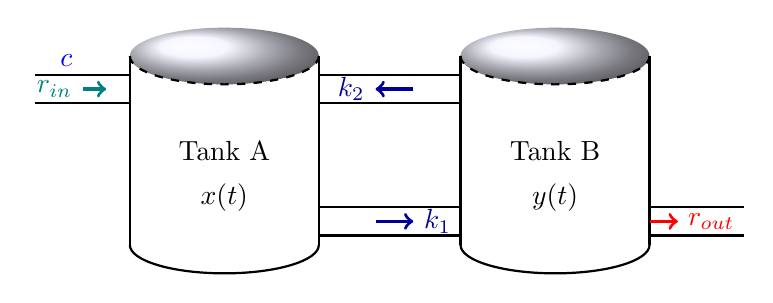
\begin{tikzpicture}[thick, scale=1.2, every node/.style={scale=1}]
				
				% Tank A
				\shade[ball color=blue!5] (0,0) ellipse (1 and 0.3); % Top ellipse
				\draw[thick] (-1,0) -- (-1,-2); % Left side
				\draw[thick] (1,0) -- (1,-2);   % Right side
				\draw[thick] (-1,-2) arc[start angle=180,end angle=360,x radius=1, y radius=0.3]; % Bottom
				\draw[dashed] (-1,0) arc[start angle=180,end angle=360,x radius=1, y radius=0.3]; % Top (dashed back)
				\node at (0,-1) { Tank A};
				\node at (0,-1.5) { $x(t)$};
				
				% Tank B
				\shade[ball color=blue!5] (3.5,0) ellipse (1 and 0.3);
				\draw[thick] (2.5,0) -- (2.5,-2);
				\draw[thick] (4.5,0) -- (4.5,-2);
				\draw[thick] (2.5,-2) arc[start angle=180,end angle=360,x radius=1, y radius=0.3];
				\draw[dashed] (2.5,0) arc[start angle=180,end angle=360,x radius=1, y radius=0.3];
				\node at (3.5,-1) { Tank B};
				\node at (3.5,-1.5) { $y(t)$};
				
				% Pipe from B to A (top)
				\draw[thick] (1, -0.2) -- (2.5, -0.2);
				\draw[thick] (1, -0.5) -- (2.5, -0.5);
				\draw[->, very thick, blue!60!black] (2, -0.35) --(1.6, -0.35)  node[left] {$k_2$};
				
			
				% Pipe from A to B (bottom)
				\draw[thick] (2.5,-1.6) -- (1,-1.6);
				\draw[thick] (2.5,-1.9) -- (1,-1.9);
				\draw[->, very thick, blue!60!black](1.6,-1.75)  -- (2,-1.75) node[right] {$k_1$};
				
				% Inflow into Tank A
				\draw[thick] (-2,-0.2) -- (-1,-0.2);
				\draw[thick] (-2,-0.5) -- (-1,-0.5);
				\draw[->, very thick, teal] (-1.5, -0.35) -- (-1.25, -0.35);
				\node[left, teal] at (-1.5, -0.35) { $r_{\text{in}}$};
				\node[left, blue] at (-1.5, -0.05) { $c$};
				
				% Outflow from Tank B
		
				\draw[thick] (4.5,-1.9) -- (5.5,-1.9);
				\draw[thick] (4.5,-1.6) -- (5.5,-1.6);
				
				\draw[->, very thick, red] (4.5, -1.75) -- (4.8, -1.75);
				\node[right, red] at (4.8, -1.75) { $r_{\text{out}}$};
			\end{tikzpicture}
			\end{figure}
		
\[\displaystyle\begin{cases}
	\displaystyle x'(t) = r_{\text{in}}\; c+\frac{k_2y(t)}{V_2+t(k_1-k_2-r_{\text{out}})}-\frac{k_1x(t)}{V_1 +t(r_{\text{in}}+k_2-k_1)},\\[3ex]
	\displaystyle y'(t) = \frac{k_1x(t)}{V_1 +t(r_{\text{in}}+k_2-k_1)}-\frac{(k_2+r_{\text{out}})y(t)}{V_2+t(k_1-k_2-r_{\text{out}})}.
\end{cases}
\]
When \(r_{\text{in}} = k_1-k_2 = r_{\text{out}},\) the system becomes

\[\displaystyle\begin{cases}
	\displaystyle x'(t) = r_{\text{in}}\; c+\frac{k_2y(t)}{V_2} - \frac{k_1x(t)}{V_1 },\\[3ex]
	\displaystyle y'(t) = \frac{k_1x(t)}{V_1}-\frac{(k_2+r_{\text{out}})y(t)}{V_2}.
\end{cases}
\]

\subsection{Coupled Spring-Mass Systems} 
Suppose that two masses $m_1$ and $m_2$ are connected to two springs $A$ and $B$   hanging vertically from  a rigid support to form a coupled spring-mass system as shown in the figure below.  
%The figure includes labels for spring constants k₁ and k₂, equilibrium positions, displacements x₁(t) and x₂(t), and restoring forces.
% with spring constants $k_1$ and $k_2$, respectively. 
% 
% 
% 	\begin{tikzpicture}[scale=1.1, every node/.style={font=\small}]
% 		
% 		% Ceiling
% 		\draw[thick] (-1,0) -- (3,0);
% 		
% 		% Spring from ceiling to mass m1
% 		\draw[decorate,decoration={coil,aspect=0.5, segment length=5pt, amplitude=4pt}] 
% 		(1.0,0) -- (1.0,-1.5);
% 		\node at (1.2,-0.8) {$\quad k_1$};
% 		
% 		% Mass m1
% 		\draw[fill=gray!20] (0.7,-1.5) rectangle (1.3,-2.0);
% 		\node at (1,-1.9) {$m_1$};
% 		
% 		% Spring from m1 to m2
% 		\draw[decorate,decoration={coil,aspect=0.5, segment length=5pt, amplitude=4pt}] 
% 		(1.0,-2.0) -- (1.0,-3.5);
% 		\node at (1.2,-2.75) {$\quad k_2$};
% 		
% 		% Mass m2
% 		\draw[fill=gray!20] (0.7,-3.5) rectangle (1.3,-4.0);
% 		\node at (1,-3.9) {$m_2$};
% 		
% 		% Equilibrium lines
% 		\draw[dashed] (-0.5,-1.7) -- (2.5,-1.7);
% 		\node[left] at (-0.5,-1.7) {\(x_1=0\)};
% 		
% 		\draw[dashed] (-0.5,-3.7) -- (2.5,-3.7);
% 		\node[left] at (-0.5,-3.7) {\(x_2=0\)};
% 		
% 		% Displacement vectors
% 		\draw[->, thick] (1.6,-1.5) -- (1.6,-1.0);
% 		\node[right] at (1.6,-1.25) {$x_1(t)$};
% 		
% 		\draw[->, thick] (1.6,-3.5) -- (1.6,-3.0);
% 		\node[right] at (1.6,-3.25) {$x_2(t)$};
% 		
% 		% Restoring force vectors
% 		\draw[->, thick, red] (1.3,-1.75) -- (1.8,-1.75);
% 		\node[right] at (1.8,-1.75) {\textcolor{red}{$-k_1 x_1$}};
% 		
% 		\draw[->, thick, red] (1.3,-3.75) -- (1.8,-3.75);
% 		\node[right] at (1.8,-3.75) {\textcolor{red}{$-k_2(x_2 - x_1)$}};
% 		
% 	\end{tikzpicture}
 	
Let $x_1(t)$ and $x_2(t)$ denote the vertical displacements of the masses from their equilibrium positions.  We take  the positive direction of the displacements to be  vertically downward.
 When the masses are in motion, the spring $B$ is subject to both a stretch and a compression, so that its net stretch of the spring $B$ is given by 
 $x_2-x_1$ when the stretch of the spring $A$ is $x_1$. Let $k_1$ and $k_2$ be the constants of proportionality in Hooke's law for the springs $A$ and $B$, respectively. We assume that there is no damping or external force acting on the masses and that weights of the springs are negligible compared to  weights of the masses.
 
  The restoring force of the spring $A$ acting on the mass $m_1$ at time $t$  is  $-k_1 x_1(t),$ and the restoring force of the spring $B$  acting on the mass $m_2$ at time $t$ is  $-k_2(x_2(t)- x_1(t)).$  In addition to the restoring force of the spring $A$, the mass $m_1$ also experiences the force of $k_2(x_2(t)- x_1(t))$ at time $t$. Suppressing $t$ in $x_1(t)$ and $x_2(t)$ and using   Newton's law,
we see that the motion of the two masses in the  spring-mass system is described by the coupled linear system
 \begin{equation}\begin{cases}\label{spring-mass-1}
 	m_1x''_1 &= -k_1 x_1 + k_2 (x_2 - x_1) = -(k_1+k_2) x_1 +k_2 x_2,\\
 	m_2 x''_2 &= -k_2 (x_2 - x_1)= k_2 x_1-k_2 x_2,
 \end{cases}
 \end{equation}
which, together with the initial conditions  $x_1(t_0) = a, x'_1(t_0) = b$, $y_1(t_0) = c, y'_1(t_0) = d,$  forms an initial value problem.  

In the next example, we solve the initial value problem (\ref{spring-mass-1}) for  $ m_1=m_2=1, k_1=3,  k_2=2,$ and $x_1(0)=0, x'_1(0)=-1, x_2(0)=0, x'_2(0)=1.$


\begin{example} Solve the second-order coupled  system of linear differential equations with initial conditions
	\begin{equation}
\begin{cases}\label{spring-mass-2}
	x_1'' = -5 x_1 + 2 x_2 , \\
	x_2'' = 2 x_1 - 2 x_2, \\
	x_1(0) = 0, \quad x_1'(0) = -1, \\
	x_2(0) = 0, \quad x_2'(0) = 1.
\end{cases}
\end{equation}
\begin{solution}
		Taking the Laplace transform yields
		
		\[
		\begin{cases}
			s^2 X_1(s) - s x_1(0) - x_1'(0) = -5 X_1(s) + 2 X_2(s), \\
			s^2 X_2(s) - s x_2(0) - x_2'(0) = 2 X_1(s) - 2 X_2(s).
		\end{cases}
		\]
		Using the given initial conditions yields	
		\[
		\begin{cases}
			(s^2+5) X_1(s) + 1 =  2 X_2(s), \\
			(s^2+2) X_2(s) - 1 = 2 X_1(s).
		\end{cases}
		\]
%		Rewrite as:
%		
%		\[
%		\begin{bmatrix}
%			s^2 + 5 & -2 \\
%			-2 & s^2 + 2
%		\end{bmatrix}
%		\begin{bmatrix}
%			X_1(s) \\ X_2(s)
%		\end{bmatrix}
%		=
%		\begin{bmatrix}
%			-1 \\ 1
%		\end{bmatrix}.
%		\]	
	Solving for $X_1(s)$ and $X_2(s)$ gives
		
		\[
		X_1(s) = \frac{-s^2}{(s^2 + 1)(s^2 + 6)} \quad \text{and}\quad  
		X_2(s) = \frac{s^2 + 3}{(s^2 + 1)(s^2 + 6)}.
		\]
		Partial fraction decomposition of $X_1(s)$ and $X_2(s)$ are
		
		\[
		X_1(s) = \frac{1/5}{s^2 + 1} - \frac{6/5}{s^2 + 6}\quad \text{and}\quad
		X_2(s) = \frac{2/5}{s^2 + 1} + \frac{3/5}{s^2 + 6}.
		\]
		Taking the inverse Laplace transform yields
		\[
			\begin{cases}
				x_1(t) &= \frac{1}{5} \sin t - \frac{6}{5 \sqrt{6}} \sin(\sqrt{6} t), \\
				x_2(t) &= \frac{2}{5} \sin t + \frac{3}{5 \sqrt{6}} \sin(\sqrt{6} t),
			\end{cases}
		\]
		which render the solutions of the given initial value problem (\ref{spring-mass-2}).
		
%\textcolor{red}{Open this figure}
		
\begin{figure}[h]
	\centering
\includegraphics[scale=.8]{chap05/Mathematica/7-6-1}
\label{chap7:fig1}
\caption{Graphs of the solutions $x_1(t)$ and $x_2(t)$}\qedhere
\end{figure}	
\end{solution}
\end{example}
 

\subsection{Electrical Network Systems}
We discussed  series and parallel $LRC$ circuits in Section~\ref{subsec:electric-circuits}. In Figure~\ref{fig:systemLRC} below,  we have an $LRC$ circuit with a voltage source  \(e(t)\). We develop a system of linear differential equations to find the charge \(q_1(t)\) on the capacitor and currents $i(t)$ and $i_2(t)$  flowing through the resistor and inductor, respectively. Let $i_1(t)$ be the current flowing through the capacitor. 


%\textcolor{red}{open the figure below}
\begin{figure}[h]
	\begin{circuitikz}[american]
		% Current source from bottom to top
		\draw
		(0,0) to[sV, invert, v_<={}, i>=${i(t)}$] (0,4)
		to[american resistor, i_=${}$, l=$R$] (2,4)
		to[short] (2.5,4); % top horizontal wire
		\node[circle, fill=white, inner sep=1pt, label=above left: Voltage source \(e(t)\)] at (-0.4,1.75) {};
		% Split point at (2,4), three parallel branches
	
		\node[circle, fill=black, inner sep=1pt, label=above right: A] at (2.5,4) {};
		% Resistor branch (left)
		\draw
		(2.5,4)
		to[C=$C$, i>_=${i_1(t)}$ ] (2.5,.2)
		-- (2.5,0); % back to bottom of source
	
		% Inductor branch (right)
		\draw
		(2.5,4) -- (4.5,4)
		to[cute inductor, l=$L$, i>_=${i_2(t)}$] (4.5,0)
		-- (4.5,0);
		% Merge point at (0,4), three parallel branches
		\node[circle, fill=black, inner sep=1pt, label=above right:] at (2.5,0) {};
		\draw
		(4.5,0)	-- (0,0); % central node
	\end{circuitikz}
	\\
	\caption{$LRC$ circuit}
	\label{fig:systemLRC}
\end{figure}

We observe that the circuit contains three distinct closed loops:
\begin{enumerate}[label= ,noitemsep]
	\item \textbf{Loop 1}: consisting of the battery, resistor, and capacitor;
	\item \textbf{Loop 2}: consisting of the battery, resistor, and inductor; and
	\item \textbf{Loop 3}: formed by the capacitor and inductor alone.
\end{enumerate}

The system of corresponding equations for the loops are:
\[
\begin{cases}
\displaystyle R\, i(t)+\frac{1}{C} q_1(t) = e(t) & \qquad\text{(for Loop 1)}\\  
\displaystyle L\, i_2'(t) + R\, i(t) = e(t)  & \qquad \text{(for Loop 2)}   \\
\displaystyle L\, i_2'(t) - \frac{1}{C} q_1(t) = 0& \qquad \text{(for Loop 3)}  
\end{cases}
\]
We observe that each equation in the system can be obtained from the remaining two. For example, the equation for Loop 2 can be obtained by adding the equations for Loop 1 and Loop 3. For  the discussion that follows, we omit the equation for Loop 2.

Furthermore, by Kirchhoff's second law, the current split at the junction A is given by  
\begin{equation*}
i(t) = i_1(t) + i_2(t),
\end{equation*}
which, in view of \( i_1(t)= q_1'(t)\), becomes

 \begin{equation*}
q'_1(t) + i_2(t) -i(t) =0.
 \end{equation*}
Thus, a linear system in $i(t), q_1(t)$ and $i_2(t)$   is

\begin{numcases}\empty
	R\, i(t)+\frac{1}{C} q_1(t) = e(t) & \qquad\text{(for Loop 1)}  \label{eq:LRC-system-1} \\
	L\, i_2'(t) - \frac{1}{C} q_1(t) = 0& \qquad \text{(for Loop 3)}  \label{eq:LRC-system-2}\\
	q'_1(t) + i_2(t) -i(t) =0  & \qquad \text{(the current split)}   \label{eq:LRC-system-3}
\end{numcases}

 
 We now proceed to solve the system \eqref{eq:LRC-system-1}-\eqref{eq:LRC-system-3}.
Differentiating \eqref{eq:LRC-system-3} with respect to $t$ yields
 \begin{equation}\label{eq:LRC-system-4}
	i'(t) = q''_1(t) + i'_2(t).
\end{equation}
Solving for $i'_2(t)$ from \eqref{eq:LRC-system-2} and substituting it into \eqref{eq:LRC-system-4} gives
 \begin{equation*}
	i'(t) = q''_1(t) + \frac{1}{LC}q_1(t).
\end{equation*}
Substituting this expression for $i'(t)$ into the equation obtained by
differentiating \eqref{eq:LRC-system-1} with respect to $t$, we get
 \begin{equation}\label{eq:LRC-system-5}
 	LRC q''_1(t) +Lq'_1(t)+ Rq_1(t) =  LCe'(t),
\end{equation}
which can be solved for $q_1(t).$   Once $q_1(t)$ is determined, we find $i_1(t)$ by using \( i_1(t)= q_1'(t).\)  We then find \(i(t)\) from \eqref{eq:LRC-system-1} by using \(q_1(t)\) there. Finally, we find $i_2(t) = i(t) - i_1(t).$

%For analogy, we can interchange the spring-mass system parameters and the \(LRC\) circuit network parameters in \eqref{eq:LRC-system-5} as follows:
%\begin{center}
%	\begin{tabular}{cccc}
%		\hline
%		Spring-Mass  &     \(LRC\) circuit    \\ \hline
%		\(m\)  &\(R\)  \\
%		\(b\)     & \(\displaystyle\frac{1}{C}\) \\[2ex]
%		\(k\)     & \(\displaystyle\frac{R}{LC}\) \\[2ex]
%		\(\omega =\sqrt{k/m}\) &\(\omega =\sqrt{1/LC}\)   \\[2ex]
%		\hline
%	\end{tabular}
%\end{center}





\begin{Exercise}\label{EX76}
	\vspace{-\baselineskip}% <-- You don't need this line of code if there's some text here
	
	\Question\label{7-6-1}
	
	
	
	
\end{Exercise}

\setboolean{firstanswerofthechapter}{true}
\begin{multicols}{2}\scriptsize
	\begin{Answer}[ref={EX75}]
		\Question \label{7-6-1a}
		\begin{tasks}
			\task
		\end{tasks} 
		
	
		
	\end{Answer}
\end{multicols}
\setboolean{firstanswerofthechapter}{false}
